%===============================================================================
% LaTeX sjabloon voor de bachelorproef toegepaste informatica aan HOGENT
% Meer info op https://github.com/HoGentTIN/bachproef-latex-sjabloon
%===============================================================================
%\tracinglostchars=3

\documentclass{bachproef-tin}

\usepackage{hogent-thesis-titlepage} % Titelpagina conform aan HOGENT huisstijl
\usepackage{xcolor}
%%---------- Documenteigenschappen ---------------------------------------------
% TODO: Vul dit aan met je eigen info:

% De titel van het rapport/bachelorproef
\title{Nursery Tone Monitor: detecteren van elderspeak via AI}

% Je eigen naam
\author{Sibian De Gussem}

% De naam van je promotor (lector van de opleiding)
\promotor{Geert Van Boven}

% De naam van je co-promotor. Als je promotor ook je opdrachtgever is en je
% dus ook inhoudelijk begeleidt (en enkel dan!), mag je dit leeg laten.
\copromotor{Jorrit Campens}

% Indien je bachelorproef in opdracht van/in samenwerking met een bedrijf of
% externe organisatie geschreven is, geef je hier de naam. Zoniet laat je dit
% zoals het is.
\instelling{---}

% Academiejaar
\academiejaar{2021-2022}

% Examenperiode
%  - 1e semester = 1e examenperiode => 1
%  - 2e semester = 2e examenperiode => 2
%  - tweede zit  = 3e examenperiode => 3
\examenperiode{2}

%===============================================================================
% Inhoud document
%===============================================================================

\begin{document}

%---------- Taalselectie -------------------------------------------------------
% Als je je bachelorproef in het Engels schrijft, haal dan onderstaande regel
% uit commentaar. Let op: de tekst op de voorkaft blijft in het Nederlands, en
% dat is ook de bedoeling!

%\selectlanguage{english}

%---------- Titelblad ----------------------------------------------------------
\inserttitlepage

%---------- Samenvatting, voorwoord --------------------------------------------
\usechapterimagefalse
%%=============================================================================
%% Voorwoord
%%=============================================================================

\chapter*{\IfLanguageName{dutch}{Woord vooraf}{Preface}}
\label{ch:voorwoord}

%% TODO:
%% Het voorwoord is het enige deel van de bachelorproef waar je vanuit je
%% eigen standpunt (``ik-vorm'') mag schrijven. Je kan hier bv. motiveren
%% waarom jij het onderwerp wil bespreken.
%% Vergeet ook niet te bedanken wie je geholpen/gesteund/... heeft

De keuze aan bachelorproefonderwerpen was omvangrijk. Ik wilde een onderwerp kiezen die een impact heeft op de maatschappij én waarbij ik Artificiële Intelligentie kon gebruiken. Enerzijds om te kunnen aantonen dat AI niet altijd een negatieve connotatie moet hebben en anderzijds omdat mijn afstudeerrichting AI \& \textit{Data Engineering} was. Op die manier kon ik te weten komen of AI \& \textit{Data Engineering} eerder iets voor mij is, of toch eerder het programmeren zelf..

Het was best wel een interessant onderwerp! Aangezien er meer en meer vergrijzing komt, is er meer nood aan ouderenzorg. Er is daarbij een duidelijk verschil tussen zorg op papier en kwalitatieve zorg in het echte leven. Ik hoop dat studenten in de opleiding verpleegkunde hierdoor minder aan \textit{elderspeak} zullen doen zodat ouderen niet behandeld worden als kleine kinderen. Hopelijk zal dit niet het geval zijn wanneer ik oud zal zijn en zorg zal nodig hebben\ldots

%TODO: hoe is het verlopen?

Het ontvangen van audiosamples was wel heel moeilijk omdat het niet zomaar een vragenlijst invullen was door wat aan te klikken, maar er werd gevraagd om zinnen in te spreken. Dit zorgde dat mensen sneller afhaakten. Toch wil ik alle 25 %TODO
mensen bedanken die me geholpen hebben om mijn systeem te testen.

Eerst en vooral wil ik mijn hogeschool, HOGENT, bedanken om zo een interessant onderwerp aan te bieden voor mijn eindwerk. Ook het feit dat dit zicht uitstrekte over twee studierichtingen heen, namelijk Toegepaste Informatica en Verpleegkunde, was een bijzondere maar leuke opstelling.

Daarnaast wil ik mijn promotor Geert Van Boven bedanken om de inhoud verschillende keren na te lezen, om mij extra informatie te geven over alle IT-onderwerpen en mij te steunen in dit proces.
Daarbij wil ik ook mijn co-promotor bedanken voor de probleemstelling duidelijk uit te leggen, voor zijn enthousiasme en zijn feedback!

Als laatste wil ik nog mijn vrienden en familie bedanken om mijn inhoud na te lezen, te verbeteren en aan te duiden wat er niet zo duidelijk was.

Dankjewel aan iedereen, zonder jullie was dit niet zo goed gelukt!
%%=============================================================================
%% Samenvatting
%%=============================================================================

% De "abstract" of samenvatting is een kernachtige (~ 1 blz. voor een
% thesis) synthese van het document.
%
% Deze aspecten moeten zeker aan bod komen:
% - Context: waarom is dit werk belangrijk?
% - Nood: waarom moest dit onderzocht worden?
% - Taak: wat heb je precies gedaan?
% - Object: wat staat in dit document geschreven?
% - Resultaat: wat was het resultaat?
% - Conclusie: wat is/zijn de belangrijkste conclusie(s)?
% - Perspectief: blijven er nog vragen open die in de toekomst nog kunnen
%    onderzocht worden? Wat is een mogelijk vervolg voor jouw onderzoek?
%
% LET OP! Een samenvatting is GEEN voorwoord!

%%---------- Nederlandse samenvatting -----------------------------------------
%
% Als je je bachelorproef in het Engels schrijft, moet je eerst een
% Nederlandse samenvatting invoegen. Haal daarvoor onderstaande code uit
% commentaar.
% Wie zijn bachelorproef in het Nederlands schrijft, kan dit negeren, de inhoud
% wordt niet in het document ingevoegd.

\IfLanguageName{english}{%
\selectlanguage{dutch}
\chapter*{Samenvatting}
\lipsum[1-4]
\selectlanguage{english}
}{}

%%---------- Samenvatting -----------------------------------------------------
% De samenvatting in de hoofdtaal van het document

\chapter*{\IfLanguageName{dutch}{Samenvatting}{Abstract}}

Deze bachelorproef behandelt het detecteren van \textit{elderspeak} a.d.h.v. een webapplicatie. \textit{Elderspeak} is het fenomeen waarbij jongere mensen tegen ouderen spreken op een betuttelende manier,  vandaar dat \textit{elderspeak} ook wel als \textit{secondary baby talk} wordt benoemd.

Hopelijk kan deze applicatie gebruikt worden bij opleidingen in de zorgsector. De studenten kunnen dit leren in een practicum waarbij ze situaties moeten naspelen. De website zal dan aangeven of er \textit{elderspeak} aanwezig is.

Dit optimaliseert de communicatie tussen zorgpersoneel en ouderen, waardoor er kan voorzien worden in een kwaliteitsvolle zorg. Op die manier is er de mogelijkheid om een waardige levenseindefase te voorzien.

Om aspecten van \textit{elderspeak} te kunnen herkennen in een gesprek, was de eerste stap het ijken van spraakherkenningssoftware met de kenmerken van \textit{elderspeak}. Spraakherkenning gebruikt achterliggend een geavanceerd artificieel intelligentie-model en daarnaast wordt \textit{natural language processing} of \textit{NLP} toegepast om de precisie te verbeteren. De spraakherkenning kan enkel werken bij een minimum aan achtergrondlawaai. Deze drie technieken worden beschreven in het literatuuronderzoek.

Nadien beschrijft deze bachelorproef hoe de applicatie van scratch opgebouwd is, welke methoden en \textit{frameworks} gebruikt worden en hoe alles met elkaar verweven werd. Zo werd een \textit{micro-framework} Flask in de programmeertaal Python gebruikt om snel een webapplicatie op te zetten. Via de Google \textit{Speech Recognition}-API en andere Python-bibliotheken kan \textit{elderspeak} gedetecteerd worden.

In het volgende hoofdstuk worden de resultaten van het testen beschreven. Zo werd er data verzameld en geïmplementeerd in een Python-script dat automatisch \textit{confusion matrixes} gebruikt om de accuraatheid van de applicatie weer te geven. Daarbij wordt er ook beschreven of er aan alle \textit{requirements} voldaan is om de applicatie af te leveren.

Als voorlaatste hoofdstuk wordt er beschreven hoe dit eindwerk kan verder evolueren en wat een mogelijk vervolg kan zijn in een multidisciplinaire omgeving. Via GitHub kan de code gedeeld worden en kan de applicatie gemakkelijk geïnstalleerd worden op een andere computer. Zo kan de applicatie geraadpleegd op een computer, maar via een parameter kunnen ook andere apparaten gebruik maken van de website.

Deze bachelorproef besluit dat het mogelijk is om \textit{elderspeak} te detecteren via AI, specifiek via spraakherkenning en Python-methoden. Dit werd gevisualiseerd op een website zodat studenten in de zorgsector beroep kunnen doen op deze tool om te oefenen.



%---------- Inhoudstafel -------------------------------------------------------
\pagestyle{empty} % Geen hoofding
\tableofcontents  % Voeg de inhoudstafel toe
\cleardoublepage  % Zorg dat volgende hoofstuk op een oneven pagina begint
\pagestyle{fancy} % Zet hoofding opnieuw aan

%---------- Lijst figuren, afkortingen, ... ------------------------------------

% Indien gewenst kan je hier een lijst van figuren/tabellen opgeven. Geef in
% dat geval je figuren/tabellen altijd een korte beschrijving:
%
%  \caption[korte beschrijving]{uitgebreide beschrijving}
%
% De korte beschrijving wordt gebruikt voor deze lijst, de uitgebreide staat bij
% de figuur of tabel zelf.

\listoffigures
\listoftables

% Als je een lijst van afkortingen of termen wil toevoegen, dan hoort die
% hier thuis. Gebruik bijvoorbeeld de ``glossaries'' package.
% https://www.overleaf.com/learn/latex/Glossaries

%---------- Kern ---------------------------------------------------------------

% De eerste hoofdstukken van een bachelorproef zijn meestal een inleiding op
% het onderwerp, literatuurstudie en verantwoording methodologie.
% Aarzel niet om een meer beschrijvende titel aan deze hoofstukken te geven of
% om bijvoorbeeld de inleiding en/of stand van zaken over meerdere hoofdstukken
% te verspreiden!

%%=============================================================================
%% Inleiding
%%=============================================================================

\chapter{\IfLanguageName{dutch}{Inleiding}{Introduction}}
\label{ch:inleiding}

De veroudering van de bevolking in de Vlaamse steden en gemeenten zet zich in de komende decennia verder.~\autocite{StatistiekVlaanderen2018}
Volgens hun voorspellingen zou tegen 2033 25\% van de bevolking een 65-plusser zijn.

Het woord `waardigheid' is actueler dan ooit.
Na de schrijnende omstandigheden van de Tweede Wereldoorlog stond dat woord centraal bij het opstellen van het verdrag van de Verenigde Naties (1945), de Universele Verklaring van de Rechten van de mens (1948) en de grondrechten van de Europese Unie (2000).
Die basiswaarde vinden we ook terug bij het Europese en Belgische zorgbeleid. Ouderen mogen niet gediscrimineerd worden op vlak van leeftijd. Tevens mogen ze ook niet op een kinderlijke, betuttelende of onvriendelijke wijze aangesproken worden en moeten ze met respect bejegend worden~\autocite{Campens21}.

Hoe meer ouderen er in de samenleving zijn, hoe meer zorg zij nodig hebben en hoe meer zorgverleners instaan voor deze leeftijdscategorie.
Die zorgverleners, maar evengoed familie, weten niet altijd even goed hoe ze moeten omgaan met senioren.
Wanneer een jonger persoon op een andere manier spreekt tegen een senior dan tegen een leeftijdsgenoot, spreken we over \textit{elderspeak}. \textcite{Williams2011} omschrijft \textit{elderspeak} als volgt: ``Elderspeak is a common intergenerational speech style used by younger persons in communication with older adults in a variety of community and health care settings. Based on negative stereotypes of older adults as less competent communicators, younger speakers (in this case nursing home staff) modify their communication with nursing home residents by simplifying the vocabulary and grammar and by adding clarifications such as repetitions and altered prosody.'' Om \textit{elderspeak} te bestrijden, gaven \textcite{Wick2007} een paar tips mee in hun onderzoek.
Enkele van die tips gingen als volgt: spreek mensen aan zoals ze wensen aangesproken te worden, vraag om ze aan te spreken met de voornaam, vermijd troetelnamen, wees bewust van non-verbaal gedrag, verhoog uw stemvolume enkel wanneer uw gesprekspartner hardhorig is, herhaal alleen uw zin als uw gesprekspartner het niet begrepen heeft, vermijd korte, langzame en makkelijke zinnen, vermijd verkleinwoorden en hanteer beleefd taalgebruik.

Naast \textit{elderspeak} heb je ook nog \textit{nursery tone}. Dit verwijst naar de situatie waarbij iemand de toonhoogte aan het einde van de zin standaard verhoogt zoals bij communicatie met jonge kinderen.

Dit onderwerp was vorig jaar al een onderzoeksonderwerp voor Glenn~\textcite{Beeckman2021} en Victor~\textcite{Standaert2021}.
Zij hebben al een basis gelegd in de goede richting om dit project tot een goed einde te brengen.
Sommige stukken programmacode van hen zullen gebruikt worden om zo een beter model op te stellen.
Zij haalden zelf ook verbeterpunten aan en moeilijkheden die, hopelijk, op te lossen zijn. Wat het verschil zal zijn tussen hun eindwerken en dit eindwerk wordt toegelicht in~\ref{sec:state-of-the-art}.

De nog steeds relevante onderzoeksvraag van dit onderwerp is: ``Kan \textit{elderspeak} gedetecteerd worden door Artificiële Intelligentie en kan dit toegepast worden in de praktijk?''. Een bijkomende onderzoeksvraag is: ``Kan \textit{nursery tone} gedetecteerd worden door Artificiële Intelligentie?''.

\color{blue}
De inleiding moet de lezer net genoeg informatie verschaffen om het onderwerp te begrijpen en in te zien waarom de onderzoeksvraag de moeite waard is om te onderzoeken. In de inleiding ga je literatuurverwijzingen beperken, zodat de tekst vlot leesbaar blijft. Je kan de inleiding verder onderverdelen in secties als dit de tekst verduidelijkt. Zaken die aan bod kunnen komen in de inleiding~\autocite{Pollefliet2011}:

\begin{itemize}
  \item context, achtergrond
  \item afbakenen van het onderwerp
  \item verantwoording van het onderwerp, methodologie
  \item probleemstelling
  \item onderzoeksdoelstelling
  \item onderzoeksvraag
  \item \ldots
\end{itemize}

\color{black}

\section{\IfLanguageName{dutch}{Probleemstelling}{Problem Statement}}
\label{sec:probleemstelling}

Dit onderzoek zal een meerwaarde moeten betekenen voor de oudere mensen in rusthuizen, homes, ziekenhuizen, maar ook nog de ouderen die zelfstandig thuis wonen. Deze mensen vinden het namelijk helemaal niet leuk om behandeld te worden als kleine kinderen. Deze applicatie zou dan \textit{elderspeak} moeten herkennen en aangeven welke eigenschappen het model gevonden heeft. Het zijn dan vooral de verpleegkundigen, dokters, maar ook familieleden die zich bewust moeten zijn hoe ze tegen ouderen praten.

\color{blue}
Uit je probleemstelling moet duidelijk zijn dat je onderzoek een meerwaarde heeft voor een concrete doelgroep. De doelgroep moet goed gedefinieerd en afgelijnd zijn. Doelgroepen als ``bedrijven,'' ``KMO's,'' systeembeheerders, enz.~zijn nog te vaag. Als je een lijstje kan maken van de personen/organisaties die een meerwaarde zullen vinden in deze bachelorproef (dit is eigenlijk je steekproefkader), dan is dat een indicatie dat de doelgroep goed gedefinieerd is. Dit kan een enkel bedrijf zijn of zelfs één persoon (je co-promotor/opdrachtgever).

\color{black}

\section{\IfLanguageName{dutch}{Onderzoeksvraag}{Research question}}
\label{sec:onderzoeksvraag}

De onderzoeksvraag die bij dit eindwerk hoort is: ``Kan \textit{elderspeak} gedetecteerd worden door Artificiële Intelligentie en kan dit toegepast worden in de praktijk?''. Een bijkomende onderzoeksvraag is: ``Kan \textit{nursery tone} gedetecteerd worden door Artificiële Intelligentie?''. Maar alleen dit beantwoorden zal uiteraard niet genoeg zijn. Het beantwoorden van de volgende deelvragen zullen wel een duidelijker en uitgebreider antwoord geven op de algemene probleemstelling:
\begin{itemize}
    \item Welk type Artificiële Intelligentie past het beste bij deze opstelling?
    \item Welk type model van \textit{machine learning} of \textit{deep learning} werkt het beste per eigenschap?
    \item Hoe zitten de Python bibliotheken in elkaar die gebruikt werden in het project?
    \item Kan je achtergrond lawaai wegfilteren en hoe precies?
    \item Zal spraakherkenning lukken met de gratis beschikbare softwarebibliotheken?
    \item Hoe zet je een ``Flask'' server op waar je \textit{webrequests} naar stuurt? En hoe verbind je daar een model mee?
\end{itemize}

\color{blue}
Wees zo concreet mogelijk bij het formuleren van je onderzoeksvraag. Een onderzoeksvraag is trouwens iets waar nog niemand op dit moment een antwoord heeft (voor zover je kan nagaan). Het opzoeken van bestaande informatie (bv. ``welke tools bestaan er voor deze toepassing?'') is dus geen onderzoeksvraag. Je kan de onderzoeksvraag verder specifiëren in deelvragen. Bv.~als je onderzoek gaat over performantiemetingen, dan
\color{black}

\section{\IfLanguageName{dutch}{Onderzoeksdoelstelling}{Research objective}}
\label{sec:onderzoeksdoelstelling}

Het resultaat van deze bachelorproef is een basiswebsite die dient als \textit{PoC} of \textit{proof-of-concept}. Die basisapplicatie vraagt eerst om gewoon te praten zoals je zou doen tegen je vrienden. Nadien wordt er gevraagd om te praten zoals je zou doen bij slechthorende senioren in een rusthuis. Om dat gevoeld te versterken zal er een foto getoond van iemand uit een rusthuis. De applicatie analyseert dan de audiosamples en geeft aan welke kenmerken er aanwezig waren van \textit{elderspeak}. Die kenmerken van \textit{elderspeak} en waarom het model `denkt' dat die eigenschappen aanwezig zijn, zijn vergaard in het literatuuronderzoek. Al de voorgaande zaken moet voor de deadline van de bachelorproef afgewerkt worden opdat het een succes kan genoemd worden.

\color{blue}
Wat is het beoogde resultaat van je bachelorproef? Wat zijn de criteria voor succes? Beschrijf die zo concreet mogelijk. Gaat het bv. om een proof-of-concept, een prototype, een verslag met aanbevelingen, een vergelijkende studie, enz.
\color{black}


\section{\IfLanguageName{dutch}{Opzet van deze bachelorproef}{Structure of this bachelor thesis}}
\label{sec:opzet-bachelorproef}

% Het is gebruikelijk aan het einde van de inleiding een overzicht te
% geven van de opbouw van de rest van de tekst. Deze sectie bevat al een aanzet
% die je kan aanvullen/aanpassen in functie van je eigen tekst.

De rest van deze bachelorproef is als volgt opgebouwd:

In Hoofdstuk~\ref{ch:stand-van-zaken} wordt een overzicht gegeven van de stand van zaken binnen het onderzoeksdomein, op basis van een literatuurstudie.

In Hoofdstuk~\ref{ch:methodologie} wordt de methodologie toegelicht en worden de gebruikte onderzoekstechnieken besproken om een antwoord te kunnen formuleren op de onderzoeksvragen.

% TODO: Vul hier aan voor je eigen hoofstukken, één of twee zinnen per hoofdstuk

In Hoofdstuk~\ref{ch:conclusie}, tenslotte, wordt de conclusie gegeven en een antwoord geformuleerd op de onderzoeksvragen. Daarbij wordt ook een aanzet gegeven voor toekomstig onderzoek binnen dit domein.
\chapter{\IfLanguageName{dutch}{Stand van zaken}{State of the art}}
\label{ch:stand-van-zaken}

% Tip: Begin elk hoofdstuk met een paragraaf inleiding die beschrijft hoe
% dit hoofdstuk past binnen het geheel van de bachelorproef. Geef in het
% bijzonder aan wat de link is met het vorige en volgende hoofdstuk.

% Pas na deze inleidende paragraaf komt de eerste sectiehoofding.


\color{blue}
Dit hoofdstuk bevat je literatuurstudie. De inhoud gaat verder op de inleiding, maar zal het onderwerp van de bachelorproef *diepgaand* uitspitten. De bedoeling is dat de lezer na lezing van dit hoofdstuk helemaal op de hoogte is van de huidige stand van zaken (state-of-the-art) in het onderzoeksdomein. Iemand die niet vertrouwd is met het onderwerp, weet nu voldoende om de rest van het verhaal te kunnen volgen, zonder dat die er nog andere informatie moet over opzoeken \autocite{Pollefliet2011}.

Je verwijst bij elke bewering die je doet, vakterm die je introduceert, enz. naar je bronnen. In \LaTeX{} kan dat met het commando \texttt{$\backslash${textcite\{\}}} of \texttt{$\backslash${autocite\{\}}}. Als argument van het commando geef je de ``sleutel'' van een ``record'' in een bibliografische databank in het Bib\LaTeX{}-formaat (een tekstbestand). Als je expliciet naar de auteur verwijst in de zin, gebruik je \texttt{$\backslash${}textcite\{\}}.
Soms wil je de auteur niet expliciet vernoemen, dan gebruik je \texttt{$\backslash${}autocite\{\}}. In de volgende paragraaf een voorbeeld van elk.

\textcite{Knuth1998} schreef een van de standaardwerken over sorteer- en zoekalgoritmen. Experten zijn het erover eens dat cloud computing een interessante opportuniteit vormen, zowel voor gebruikers als voor dienstverleners op vlak van informatietechnologie~\autocite{Creeger2009}.

\color{black}

\section{Verkennend onderzoek}
\label{sec:verkennend-onderzoek}
``Kan \textit{elderspeak} gedetecteerd worden door Artificiële Intelligentie en kan dit toegepast worden in de praktijk?'', is de centrale onderzoeksvraag, maar daarvoor moeten we twee begrippen goed uitleggen en begrijpen om te kunnen staven of dit wel degelijk mogelijk is.
Er zal dus eerst beschreven worden wat \textit{elderspeak} precies is. Waarom vinden ouderen dat niet leuk? Wat zijn de eigenschappen en hoe kan je het voorkomen?
Daarnaast moeten we ook begrijpen wat Artificiële Intelligentie is met daarbij alle verschillende types, vormen en maten ervan. De reden hiervoor is dat er verstaan moet worden welke en hoe AI gebruikt werd in het eindresultaat.

\section{Elderspeak}

\subsection{Wat is \textit{Elderspeak}?}

Het begrip \textit{elderspeak}, ook \textit{secondary babytalk} genoemd, kent verschillende definities. \textcite{Kemper1998} omschrijft het begrip als volgt:
``Elderspeak is a simplified speech register with exaggerated pitch and intonation, simplified grammar, limited vocabulary and slow rate of delivery.''

Daarnaast beschrijft \textcite{Williams2011} het begrip als het volgende:
``Elderspeak is a common intergenerational speech style used by younger persons in communication with older adults in a variety of community and health care settings. Based on negative stereotypes of older adults as less competent communicators, younger speakers (in this case nursing home staff) modify their communication with nursing home residents by simplifying the vocabulary and grammar and by adding clarifications such as repetitions and altered prosody.'' Dus het gaat over stereotype communicatie tussen ouderen en jongeren zoals het vereenvoudigen van zinnen en het toevoegen van herhalingen.

\subsection{Wat zijn de kenmerken?}
Deze kenmerken komen overeen met een communicatiestijl die men hanteert wanneer men tegen (afhankelijke) kinderen praat. Vandaar dat \textit{elderspeak} ook wel als \textit{secondary baby} talk wordt benoemd. \textcite{Campens2021} volgende de kenmerken als volgt op:

\begin{itemize}
    \item Langzaam spreken
    \item Verhoogde toonhoogte
    \item Verhoogd stemvolume
    \item Overdreven intonatie
    \item Vereenvoudigd woordgebruik, gebruik van verkleinwoorden en/of ongepaste bijnamen of troetelnamen
    \item Verminderde grammaticale complexiteit (bv. voornamelijk enkelvoudige zinnen)
    \item Gebruik van collectieve voornaamwoorden (bijvoorbeeld ``we'' in plaats van ``jij'')
    \item Veelvuldig gebruik van (bevestigende) tussenwerpsels (zoals ``hé'' of ``voilà'')
    \item Gewijzigd non-verbaal gedrag (bv. langdurig oogcontact, extra gebaren, te dichtbij komen)
    \item Veelvuldige verduidelijking en herhaling
\end{itemize}

Tenslotte is het belangrijk om te weten dat bij \textit{elderspeak} de inhoud van de boodschap, die de zorgverlener wil overbrengen, niet wijzigt. Wel verandert de wijze waarop de boodschap wordt overgebracht door het gebruik van een infantiliserende communicatiestijl, aldus \textcite{Campens2021}.

\subsection{Wat zijn de tips om \textit{elderspeak} te voorkomen?}

De onderstaande tips zijn enkele van de tips die \textcite{Wick2007} meegeven ter voorkoming van \textit{elderspeak}:

\begin{itemize}
    \item Spreek personen aan met de naam waarmee ze willen aangesproken worden. Gebruik geen collectieve voornaamwoorden als die niet van toepassing zijn.
    \item Als een persoon een zorgverlener toelaat om hem of haar met zijn voornaam aan te spreken, ga er dan niet van uit dat deze “toestemming” voor alle zorgverleners geldt. De mate van intimiteit varieert, waardoor elke zorgverlener moet nagaan hoe hij of zij zijn gesprekspartner mag aanspreken.
    \item Vermijd het gebruik van troetelnamen en overmatige intieme liefkozingen, tenzij de gesprekspartner uitdrukkelijk aangeeft dat hij of zij zo wil aangesproken worden.
    \item Wees je bewust van je non-verbaal gedrag.
    \item Verhoog je stemvolume (in beperkte mate) enkel en alleen wanneer de gesprekspartner hardhorig is. Verhoging van je stemvolume betekent geen verhoging van je stemhoogte. Wees je ervan bewust dat niet elke oudere gesprekspartner hardhorig is.
    \item Herhaling en verminderde grammaticale complexiteit hebben een plaats als de gesprekspartner je niet begrepen heeft.
    \item Vermijd korte zinnen en langzaam en met overdreven intonatie uitgesproken zinnen.
    \item Vermijd het gebruik van verkleinwoorden, aangezien die het gevoel van afhankelijkheid kunnen versterken en denigrerend kunnen geïnterpreteerd worden.
    \item Vermijd overdreven directieve boodschappen en bied keuzevrijheid.
    \item Hanteer een beleefd taalgebruik en beleefde omgangsvormen (bv. op de kamerdeur kloppen alvorens de kamer binnen te gaan).
\end{itemize}

\clearpage

\section{Artificiële Intelligentie}
\subsection{Wat is AI?}
Er zijn bijzonder veel beschrijvingen van wat AI is, maar alleen uit verschillende bronnen kan je een accuraat beeld krijgen van wat AI precies is.

Volgens \textcite{Oracle2014} heeft AI (kunstmatige intelligentie) betrekking op systemen of machines die onze eigen intelligentie nabootsen om taken uit te voeren en die zichzelf tijdens dat proces kunnen verbeteren op basis van de vergaarde informatie.

Het \textcite{EuropeesParlement2020} geeft de volgende definitie aan artificiële intelligentie (of kunstmatige intelligentie): ``AI is de mogelijkheid van een machine om mensachtige vaardigheden te vertonen - zoals redeneren, leren, plannen en creativiteit.
AI maakt het voor technische systemen mogelijk om hun omgeving waar te nemen, om om te gaan met deze waarnemingen en problemen op te lossen om een specifiek doel te bereiken. De computer ontvangt data - reeds voorbereid en verzameld via eigen sensoren, zoals een camera - verwerkt deze en reageert erop.
AI-systemen zijn in staat om hun gedrag in zekere mate aan te passen door het effect van vorige acties te analyseren en autonoom te werken.''

Samengevat is AI een technisch systeem dat opereert via complexe/grootschalige informatievergaring, maar waarbij het systeem vooral ook zichzelf aanpast op basis van die vergaarde informatie en op die manier menselijke intelligentie nabootst.

\subsection{Welke vormen zijn van AI?}
Artificiële Intelligentie is een verzamelnaam voor twee soorten algoritmes. Zo is er enerzijds \textit{machine learning} en anderzijds \textit{deep learning}~\autocite{Kavlakoglu2020}.
Dit kan mooi geïllustreerd worden a.d.h.v.\ figuur~\ref{fig:soorten_ai_diagram}. Daarop kan er afgeleid worden dat Artificiële Intelligentie een verzamelnaam is. Specifieker is er dan \textit{machine learning} en \textit{deep learning}.

\begin{figure}
    \centering
    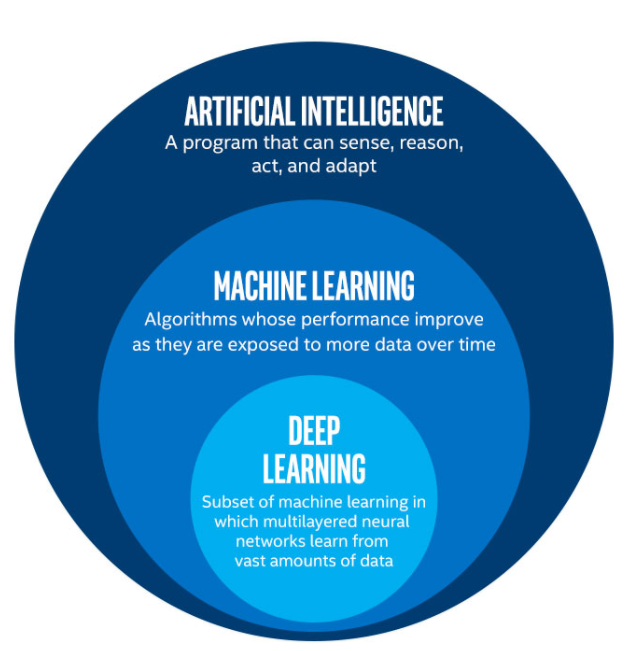
\includegraphics[width=0.6\textwidth]{./img/ai_fields.png}
    \caption{\label{fig:soorten_ai_diagram} Soorten AI in diagram~\autocite{Bansal2019}}
\end{figure}

\subsection{\textit{Machine learning}}
\textit{Machine learning} of machinaal leren is het deelgebied van kunstmatige intelligentie dat computers het vermogen geeft te leren zonder expliciet geprogrammeerd te zijn, aldus \textcite{Lievens2021}. Machinaal leren heeft drie types namelijk \textit{supervised learning} of gesuperviseerd leren, \textit{unsupervised learning} of leren zonder toezicht en als laatste type is er \textit{reinforcement learning} of leren door bekrachtiging.

\subsubsection{Supervised learning}
Een defenitie gegeven door \textcite{Lievens2021} over \textit{supervised learning} gaat als volgt: ``De taak van \textit{supervised learning} is een hypothese op te bouwen op basis van een reeks gelabelde trainingsgegevens. Deze hypothese kan dan worden gebruikt om het label voor een (nieuwe) input te voorspellen. Wanneer het label een reëel getal is, spreekt men van een regressieprobleem; wanneer het label beperkt is tot een (beperkt) aantal vooraf gedefinieerde klassen, wordt het probleem een classificatieprobleem genoemd.''
De visuele voorstelling van beide problemen is te vinden in figuur~\ref{fig:classification_vs_regression}.

Een voorbeeld van het regressieprobleem is het voorspellen van huisprijzen. De input van het model is dan een reeks vectoren die de eigenschappen van het huis voorstellen zoals aantal slaapkamers, oppervlakte, bouwjaar etc.

Voorbeelden van het classificatieprobleem zijn spamdetectie, nummerherkenning of diabetes. Elk hebben ze een beperkt aantal output klassen. Bij spamdetectie zijn er twee vooraf gedefinieerde klassen: spam en geen spam. Bij het herkennen van nummers zijn er 10 klassen: 0 t.e.m. 10 en bij diabetesdetectie kunnen er drie klassen aanwezig zijn namelijk geen diabetes, diabetes en pre-diabetes.

\begin{figure}
    \centering
    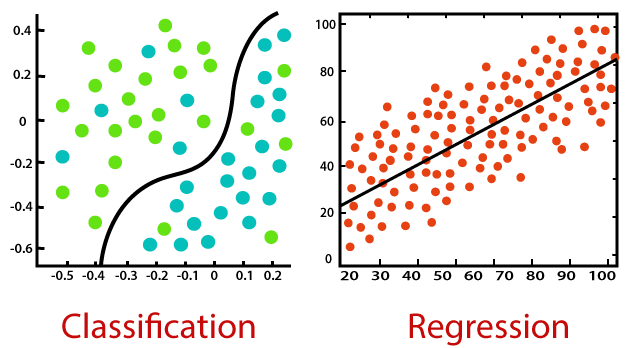
\includegraphics[width=0.75\textwidth]{./img/classification_regression.png}
    \caption{\label{fig:classification_vs_regression} Classification vs. Regression~\autocite{JavaTpoint2021}}
\end{figure}

\subsubsection{Unsupervised learning}
\textcite{Lievens2021} omschrijft \textit{unsupervised learning} als de taak van het ontdekken van structuur in een ongelabelde gegevensreeks.

De meest prominente taak bij \textit{unsupervised learning} is \textit{clustering}, d.w.z.\ de ontdekking van coherente
groepen. Andere mogelijke taken zijn anomaliedetectie en hoofdcomponentenanalyse (PCA).

Een voorbeelden van clustering is marktsegmentatie waarbij klanten worden opgedeeld in verschillende segmenten zoals trouwe klant, mogelijke vertrekkende klant, niet tevreden klant etc. Op basis van aankoopdata, tijdstippen en online activiteit kan men de klanten gaan indelen in clusters. Die informatie kan dan weer gebruikt worden om bepaalde clusters meer informatie te geven of korting te geven.
Er zijn algoritmen die fraude opsporen op een website die anders gedrag dan normaal gaan detecteren, wat dan een voorbeeld van anomalie detectie is.
Bij PCA worden de data gereduceerd zodat de minder relevante data afneemt in de dataset, maar de nodige data juist duidelijker maakt.


\subsubsection{Reinforcement learning}
\textcite{Lievens2021} beschrijft leren door bekrachtiging door een techniek die niet echt een dataset gebruikt, maar eerder via een identiteit is die leeft in een (on)bekende wereld. Die identiteit krijgt dan beloningssignalen. De opdracht is dan om uit te zoeken wat de regels zijn die leiden tot een grote beloning.

Het bekendste voorbeeld van \textit{reinforcement learning} is zelfrijdende wagens waarbij het model alles zelf moet aanleren zoals het remmen en gas geven in welke hoeveelheid en hoe er gestuurd moet worden. Dit is een lang en iteratief proces waarbij het model dus de hele tijd zichzelf bijstuurt en bijleert van wat het net gezien heeft.

\subsection{\textit{Deep Learning}}
\textit{Deep learning} is een onderdeel van \textit{machine learning} die neurale netwerken bevat.
``Een artificieel neuraal netwerk bestaat uit een groot aantal eenvoudige rekende eenheden, units of neuronen die de volgende eigenschap heeft: `Als de (gewogen) input van een neuron groot is, zal het 'vuren' en dit neuron zal een grote waarde op zijn axon zetten. Bovendien zijn deze eenheden verbonden door middel van gerichte links waarbij een reëel getal de sterkte van elke verbinding aangeeft.'', aldus \textcite{Lievens2021} in zijn cursus \textit{Distributed Databases}.

De systematische voorstelling van een neuron is te vinden in figuur~\ref{fig:neuron}.
Een volledig neuraal netwerk kan er uit zien zoals in figuur~\ref{fig:layers}. De data wordt gevoed aan de \textit{input layer}. Daarna komen een x-aantal \textit{hidden layers} die dan de bewerkingen uitvoeren en als laatste stap heb je de \textit{output layer}. Het aantal \textit{nodes} of knopen in de \textit{output layer} is gelijk aan het aantal klassen die een probleem heeft. Als er een \textit{deep learning} model gemaakt wordt van het detecteren van spam, dan zou de \textit{output layer} twee knopen moeten hebben.

\begin{figure}
    \centering
    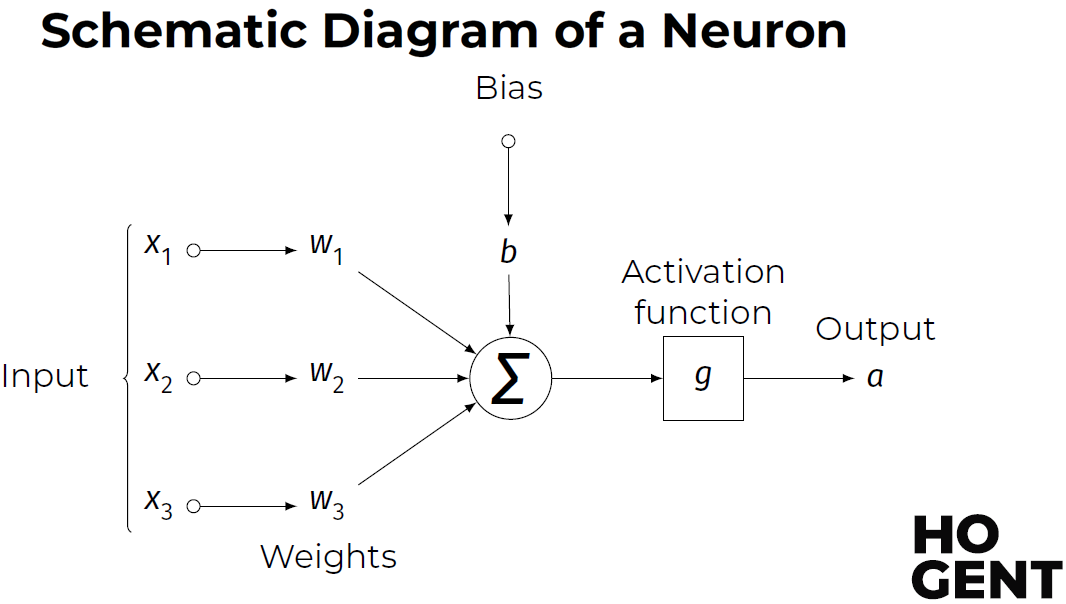
\includegraphics[width=1\textwidth]{./img/neuron}
    \caption{\label{fig:neuron} Systematische voorstelling van een Neuron~\autocite{Lievens2021}}
\end{figure}

\begin{figure}
    \centering
    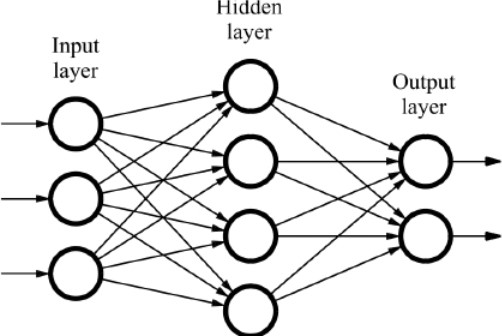
\includegraphics[width=.5\textwidth]{./img/layers}
    \caption{\label{fig:layers} Layers van een artificieel neuraal netwerk~\autocite{Lievens2021}}
\end{figure}

\subsection{AI in het dagelijkse leven: TODO: misschien weglaten?}
Om een klein overzicht te maken wat AI allemaal inhoudt, zijn er andere voorbeelden geïllustreerd van kunstmatige intelligentie in figuur~\ref{fig:ai_dagelijkse_leven}.
TODO: meer informatie geven of weglaten?

\begin{figure}
    \centering
    
\includegraphics[width=.8\textwidth]{./img/ai_voorbeelden}
    \caption{\label{fig:ai_dagelijkse_leven} AI in het dagelijkse leven.~\autocite{EuropeesParlement2020}}
\end{figure}

\section{AI-technieken die gebruikt worden om elderspeak te detecteren}

\subsection{NLP of \textit{natural language processing}}
Om te kunnen detecteren of men verkleinwoorden, troetelnamen, collectieve voornaamwoorden of veel tussenwerpsels gebruikt, moet het model of eerder gezegd de Python-bibliotheek - die het model bevat - weten of deze eigenschappen voorkomen. Hiervoor moeten we gebruik maken van \textit{natural language processing}-bibliotheken of kort NLP. Maar wat is NLP precies?

\textit{Natural language processing} of vertaald ``natuurlijke taalverwerking'' zit in de tak van de kunstmatige intelligentie. NLP zit een stuk in \textit{machine learning} en een stukje in \textit{deep learning}.~\autocite{Kleinings2022} De visuele voorstelling van die verhoudingen zijn te vinden in figuur \ref{fig:nlp_field}.

Volgens \textcite{Kleinings2022} is die natuurlijke taalverwerking een technologie die gebruikt wordt om computers te helpen om natuurlijke menselijke taal te begrijpen en te interpreteren.

NLP combineert computationele linguïstiek - op regels gebaseerde modellering van menselijke taal - met statistische, \textit{machine learning}- en \textit{deep learning}-modellen. Samen stellen deze technologieën computers in staat menselijke taal - in de vorm van tekst of spraakgegevens - te verwerken en de volledige betekenis ervan te ``begrijpen'', compleet met de bedoeling en het sentiment van de spreker of schrijver.~\autocite{IBMCloudEducation2021}

NLP stuurt computerprogramma's aan die tekst van de ene taal naar de andere vertalen, reageren op gesproken opdrachten en grote hoeveelheden tekst kan samengevat worden, zelfs in realtime. Enkele voorbeelden van NLP-systemen in het dagelijkse leven zijn: spraakgestuurde GPS-systemen, digitale assistenten, spraak-naar-tekst dicteersoftware in bijvoorbeeld de smartphone of Microsoft Word, chatbots voor de klantenservice en andere `gemakken' voor de consument. Maar NLP speelt ook een steeds grotere rol in bedrijfsoplossingen die helpen bij het stroomlijnen van de bedrijfsvoering, het verhogen van de productiviteit van werknemers en het vereenvoudigen van bedrijfskritische bedrijfsprocessen, aldus \textcite{IBMCloudEducation2021}.

\begin{figure}
    \centering
    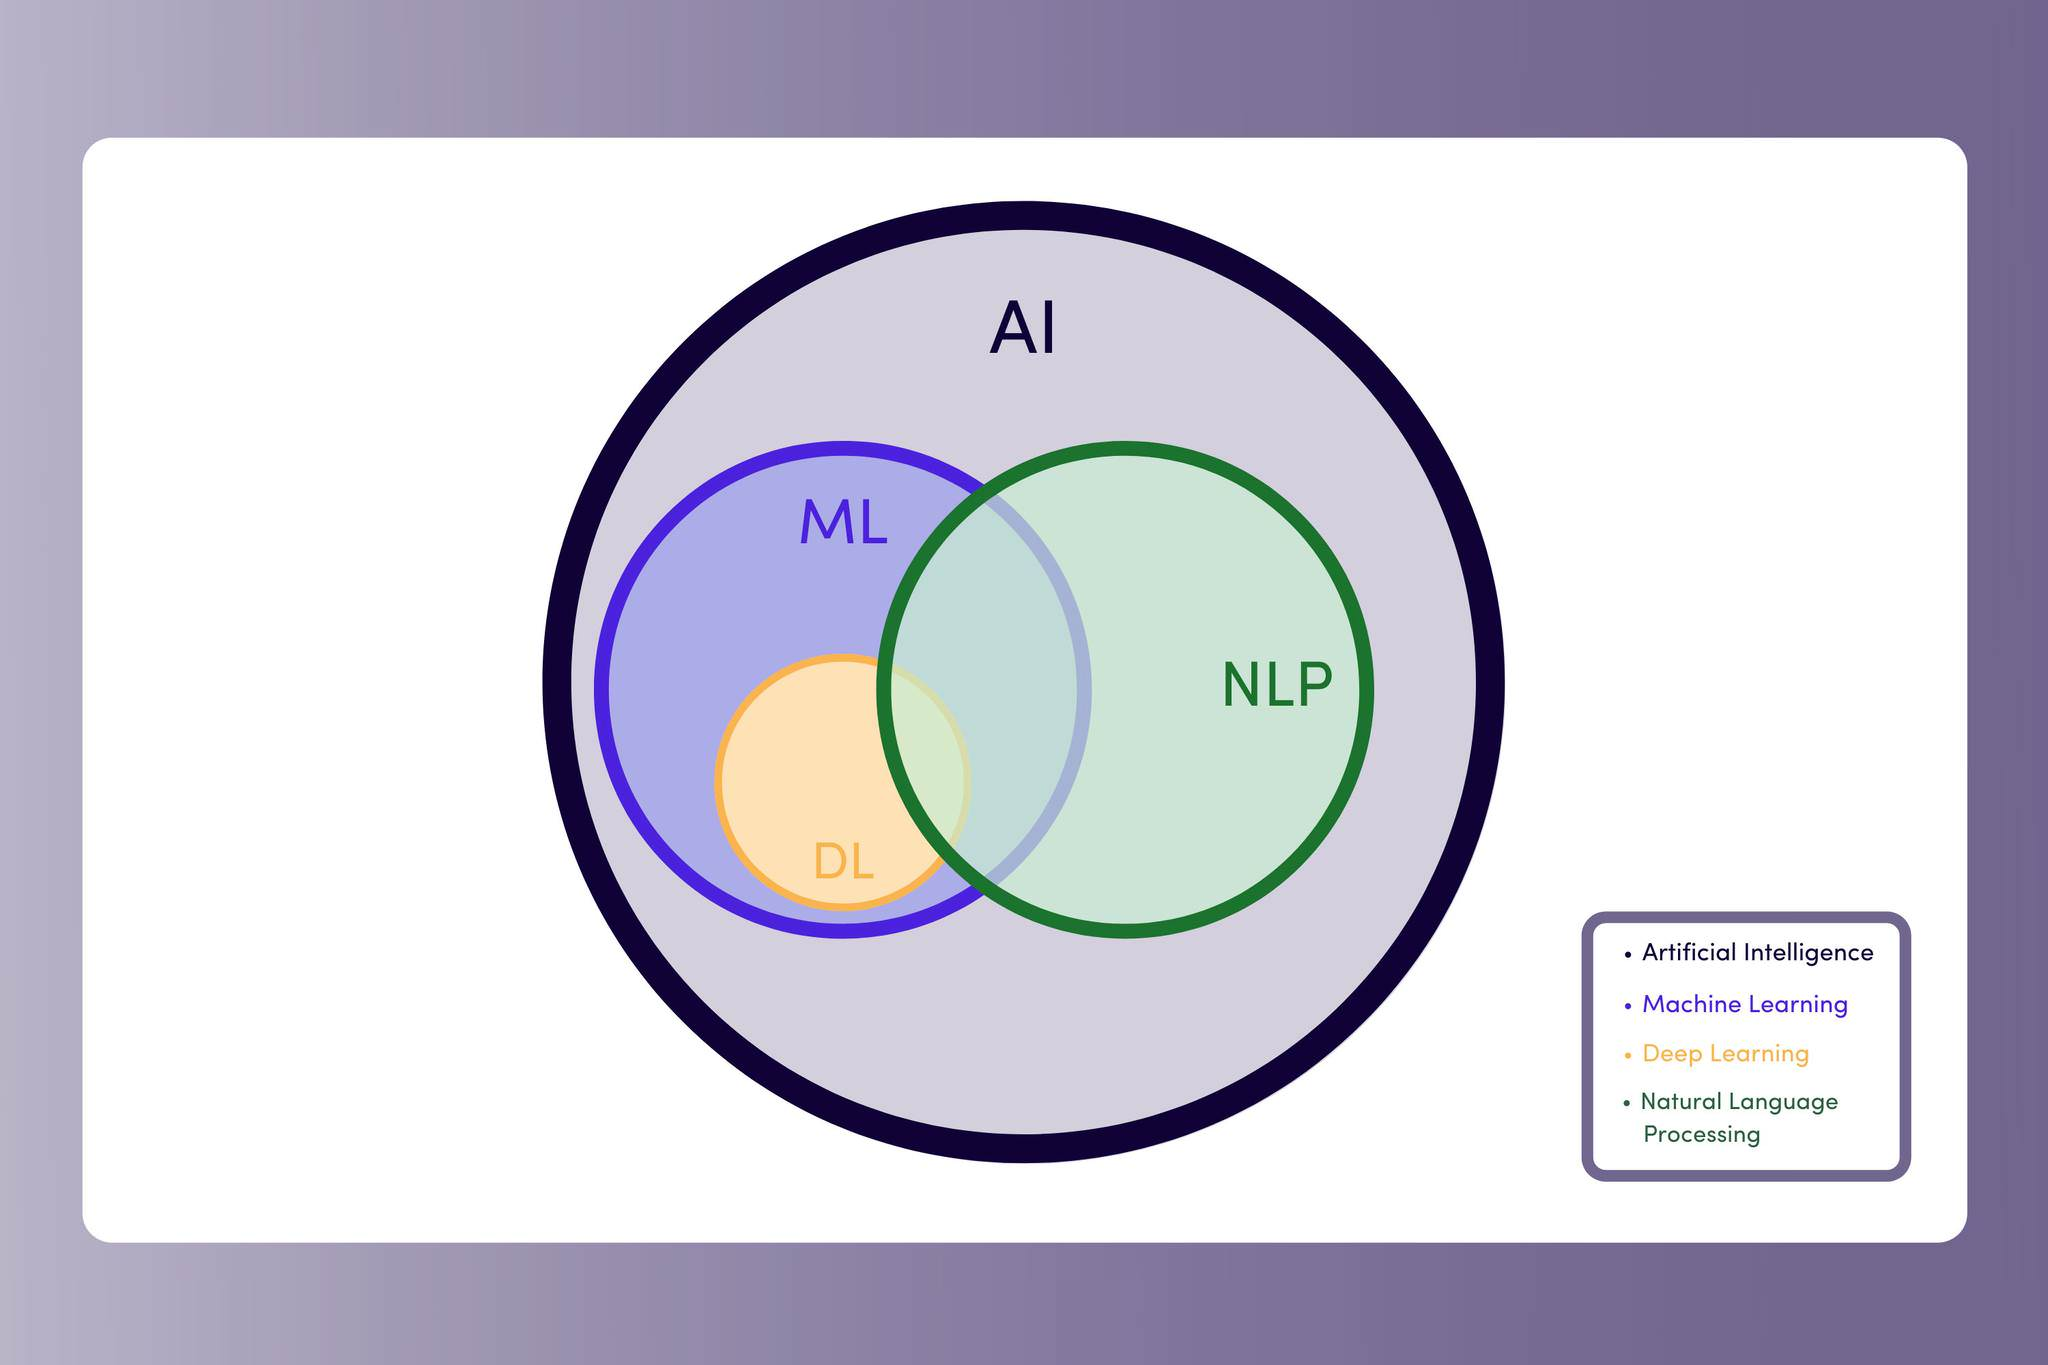
\includegraphics[width=.8\textwidth]{./img/nlp_field_ai.jpeg}
    \caption{\label{fig:nlp_field} Situering van NLP binnen het AI-veld.~\autocite{Kleinings2022}}
\end{figure}

\subsubsection{Waarom is het analyseren van taal moeilijk?}
Volgens \textcite{Kleinings2022} zijn er vele redenen waarom het verwerken van taal door een computer of AI-systeem nog steeds moeilijk is en zal blijven.

Eerst en vooral heb je alle linguïstische regels per taal. Zo zijn er meer dan 6500 talen die gesproken worden vandaag de dag, die elke hun aparte regels hebben.
Daarnaast is er het probleem van de uniformiteit. Om taal te kunnen verwerken moet die eerst omgezet worden in een systeem of formaat dat de computer kan begrijpen. Door middel van machinaal leren identificeert het model ongestructureerde taal en zet deze om naar bruikbare, niet dubbelzinnige informatie die de computer dan kan begrijpen en er verder mee kan rekenen. Dit stukje wordt de \textit{pre-processing} genoemd.

Bovendien speelt de context ook vaak parten. \textit{Natural Language Processing} werkt fundamenteel door de hiërarchie van linguïstische dictie tussen elk woord te begrijpen en deze om te zetten in een vorm die computers kunnen interpreteren. Onze talen zijn niet eenvoudig, zo hebben woorden meerdere betekenissen, die alleen begrepen worden door het verschil in context.~\autocite{Kleinings2022} Een voorbeeld hiervan is het woord ``bank''. In de ene context is het de financiële instelling en in een andere context is het de rustbank in het park.
Als laatste kan de toon van de stem ook nog verschillen. Mensen kunnen sarcasme of ironie in hun taal steken zodat het een andere betekenis krijgt. Om deze andere betekenis uit een tekst te halen is er heel veel moeite voor nodig.

\subsubsection{Hoe werkt NLP?}
NLP is niet één statische methode, maar een ketting van manipulaties van de tekst zodat er meer lagen informatie tevoorschijn komen. Dit wordt gerealiseerd met neurale netwerken waarbij elke node een bepaalde functie uitvoert.
Er zijn vier grote stappen i.v.m. de taalverwerking: morfologie, syntaxis, semantiek en pragmatiek, schrijft \textcite{Kleinings2022}, wat te lezen is op een \textit{low-code/no-code} platform genaamd Levity die dus veel kennis hebben over AI. Daar kan men blokken slepen en gebruiken om een AI-model op te stellen.

Met behulp van morfologie kan er per woord een type geclassificeerd worden zoals een zelfstandig naamwoord, bijvoeglijk naamwoord, voornaamwoord, lidwoord enzovoort. Denk hierbij aan het voorbeeld met de bank.

Om de syntaxis aan te leren zijn er twee manieren. Enerzijds kunnen er woorden gelabeld worden waarbij er gezegd wordt dat woord A de stam is, woord B de 2e persoon enkelvoud, woord C het voltooid deelwoord etc. Anderzijds kan er een \textit{unsupervised machine learning} model gemaakt worden waarbij de computer de regels afleidt uit verschillende gelabelde teksten en die logica gebruikt om nieuwe, niet-gelabelde, teksten te begrijpen met dezelfde logica.

Daarnaast is het ook aan te raden dat stopwoorden verwijderd worden als het model de tekst wil begrijpen. Stopwoorden zoals ``een, de, euh, inderdaad, echt, oké, eigenlijk, allez, etc.'' moeten verwijderd worden. Daarbij aansluitend zijn er twee andere methoden. Enerzijds lemmatiseren waarbij  werkwoorden naar de tegenwoordige tijd veranderd worden, en anderzijds stemming, waarbij er prefixen of affixen verwijderd worden, ook nodig om de conversie te maken. Een voorbeelden van het converteren is dan: ``wij dachten'' naar ``denk''. Woorden worden daarnaast ook vervangen door meer gebruikte synoniemen zoals van ``enorm'' naar ``groot''.

Als laatste systeem of layer bestaat er \textit{tokenization}. Dit is het proces waarbij het systeem de zin indeelt in verschillende eenheden waaruit informatie kan gehaald worden.
Er kan een \textit{token} gekozen worden op basis van regels, leestekens, spaties, maar dit geeft wel steeds een ander resultaat wat geïllustreerd is in figuur \ref{fig:tokens}. Hoe die \textit{tokenization} zich verhoudt met die layer van het \textit{deep learning} NLP model is te vinden in figuur \ref{fig:tokens_verhouding_dl}.

\begin{figure}
    \centering
    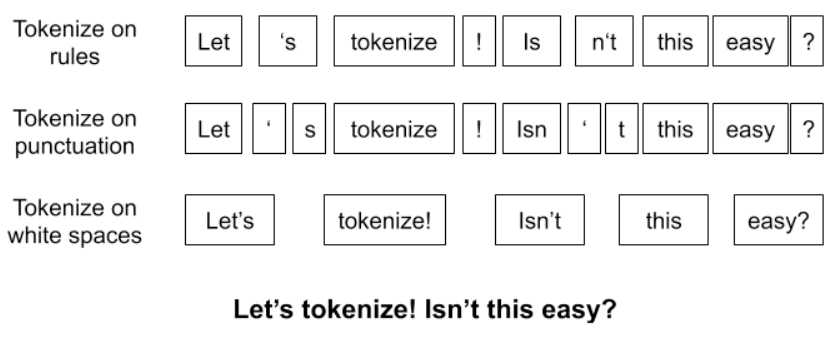
\includegraphics[width=1\textwidth]{./img/tokenize_manier}
    \caption{\label{fig:tokens} Manieren om een zin om te delen volgens een \textit{token}.~\autocite{Horan2020}}
\end{figure}

\begin{figure}
    \centering
    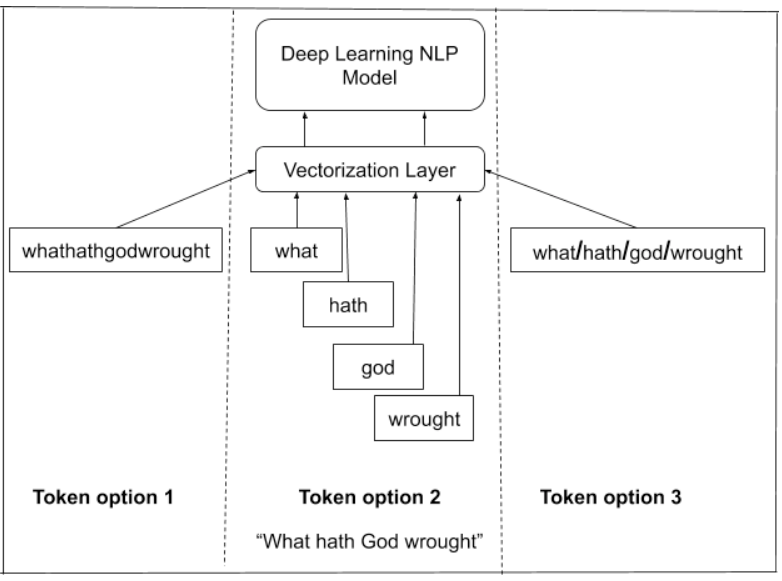
\includegraphics[width=0.8\textwidth]{./img/tokenization-1}
    \caption{\label{fig:tokens_verhouding_dl}Verhouding \textit{deep learning} NLP model met de layers en de verschillende \textit{tokens}.~\autocite{Horan2020}}
\end{figure}

\clearpage

\subsection{Filteren van achtergrond lawaai}
Volgens \textcite{Jung2021} helpen \textit{convolutional neural networks} of CNN's - een specifieke opstelling van een \textit{deep learning} model waarbij een
data-array van twee of meer dimensies, zoals een afbeelding of geluidsfragment, wordt gestapeld door een veelvoud van tweedimensionale filters - bijzonder veel om achtergrondlawaai weg te filteren.

Om achtergrond lawaai weg te werken zijn AI gebaseerde filters zoals de \textit{short-time Fourier transform} of STFT ideaal. De STFT-filter verbetert in het algemeen de kwaliteit van het inkomende geluidssignaal door ruis uit het geluidssignaal te verwijderen.
De STFT is een Fourier-gerelateerde transformatie die wordt gebruikt om de sinusoïdale frequentie- en fase-inhoud van plaatselijke delen van een signaal te bepalen terwijl dit in de tijd verandert, zie figuur~\ref{fig:conversion}. In de praktijk worden STFT's berekend door een tijdsignaal op te delen in kortere segmenten van gelijke lengte en de Fouriertransformatie afzonderlijk te berekenen voor elk korter segment. Aldus wordt het Fourier-spectrum voor elk korter segment onthuld. Gewoonlijk zet men dan de veranderende spectra
als functie van de tijd;
de grafiek staat bekend als een spectrogram of watervalgrafiek, zie figuur~\ref{fig:The_original_noise-removed_audio}.~\autocite{Jung2021}

\begin{figure}
    \centering
    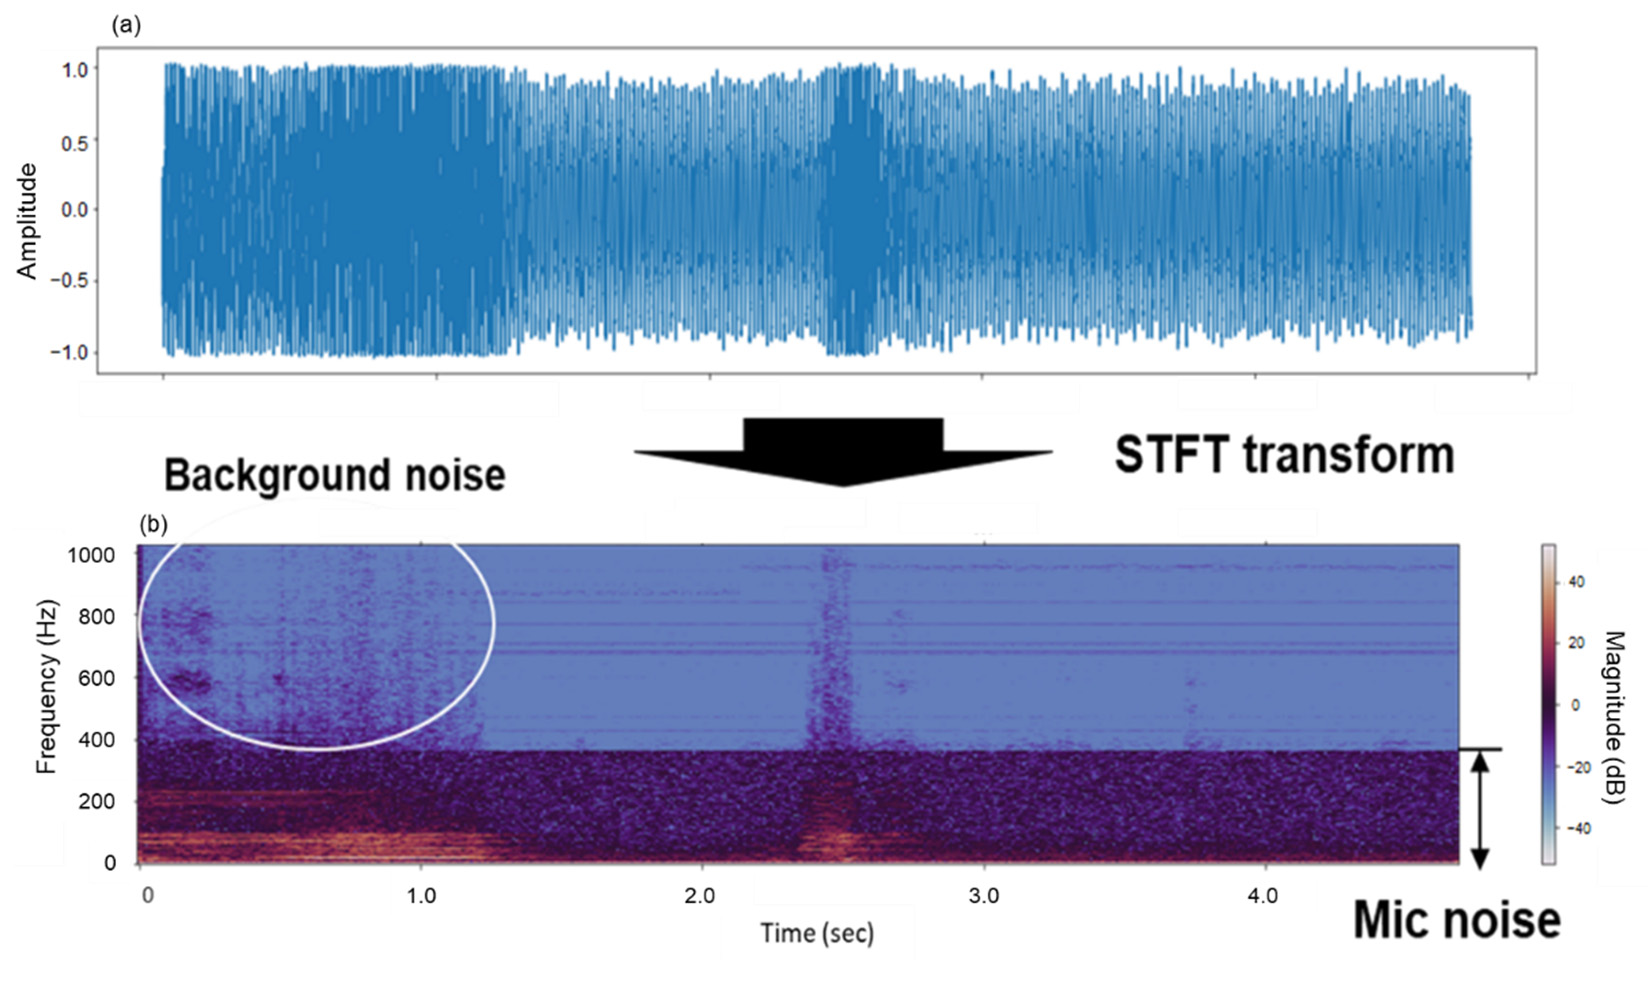
\includegraphics[width=0.8\textwidth]{./img/conversion.jpg}
    \caption{\label{fig:conversion}Tweedimensionale bron van de spraakgegevens van de oestrusoproep bij runderen (a) en de omzetting naar korte-tijd Fourier transform (STFT) gebied (b).~\autocite{Jung2021}}
\end{figure}

\begin{figure}
    \centering
    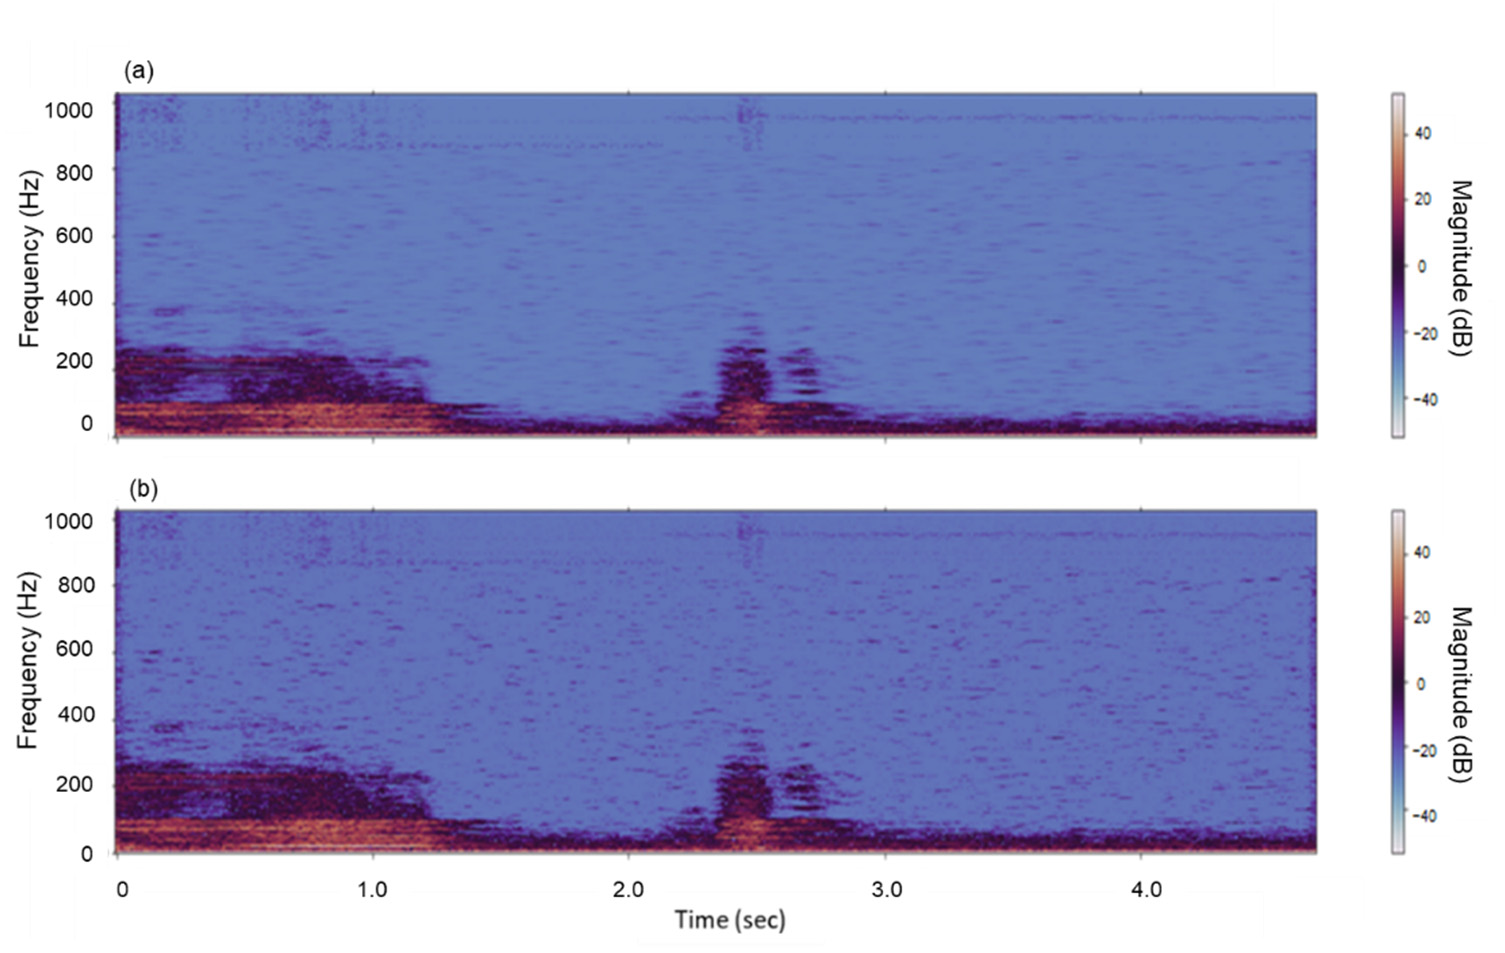
\includegraphics[width=0.8\textwidth]{./img/The_original_noise-removed_audio.jpg}
    \caption{\label{fig:The_original_noise-removed_audio}De originele audio met ruisonderdrukking (a) en spraakinformatie gecorrigeerd door ruismasker afvlakking (b).~\autocite{Jung2021}}
\end{figure}

In de opstelling van het onderzoek van \textcite{Jung2021} gebruikte men de \textit{librosa} en de \textit{noisereduce} Python-bibliotheken. Deze twee bibliotheken zullen ook gebruikt worden in het praktische gedeelte van deze bachelorproef.

%%=============================================================================
%% Methodologie
%%=============================================================================

\chapter{\IfLanguageName{dutch}{Methodologie}{Methodology}}
\label{ch:methodologie}

%% TODO: Hoe ben je te werk gegaan? Verdeel je onderzoek in grote fasen, en
%% licht in elke fase toe welke stappen je gevolgd hebt. Verantwoord waarom je
%% op deze manier te werk gegaan bent. Je moet kunnen aantonen dat je de best
%% mogelijke manier toegepast hebt om een antwoord te vinden op de
%% onderzoeksvraag.

Na het literatuuronderzoek dat uitgeschreven is in de stand van zaken over wat \textit{elderspeak} en \textit{nursery tone} precies zijn, is het doel van deze bachelorproef om een website te ontwikkelen waarmee er \textit{elderspeak} kan gedetecteerd worden via een detector. In het literatuur werd er ook theoretisch beschreven wat AI is en welke types er zijn, wat en hoe \textit{natural language processing} werkt en hoe men achtergrond lawaai filtert.

Alle eigenschappen van \textit{elderspeak} worden herkend a.d.h.v. Python-bibliotheken en niet op basis van een zelf gemaakt AI-model. De reden hiervoor is dat men het warm water niet opnieuw moet uitvinden. Zo staafde \textcite{Beeckman2021} het volgende over zelf een AI-model te maken voor deze opstelling: ``Deze bachelorproef heeft geen meerwaarde kunnen aantonen voor het gebruik van een CNN. Wegens omstandigheden was het niet mogelijk te beschikken over een grote dataset wat leidt tot slechte voorspellingen van het model. Het model voorspelt een classificatie aan dezelfde accuraatheid dan dat gokken zou teweegbrengen. Dit maakt het huidige model onbruikbaar in de praktijk.''. Door deze bewering is de denkpiste in combinatie met de kleine dataset, die in dit onderzoek verzameld werd, over zelf een AI-model opstellen al snel van tafel geveegd. Ook de promotor Van Boven haalde aan dat er genoeg Python-bibliotheken ter beschikking waren om de opdracht op die manier tot een goed einde te brengen.

Sommige methoden konden gekopieerd worden van de bijlagen van de studenten die hiervoor aan gewerkt hebben, maar niet alle code stond beschreven in die bijlage. Daarnaast had \textcite{Standaert2021} geen GitHub-\textit{repository} waardoor de code niet snel kon hergebruikt worden. Ook zaten er af en toe kleine foutjes in de code waarbij het nodig was om die op te lossen. Daardoor zal er in Hoofdstuk~\ref{ch:vervolg} een deeltje aanbod komen over waarom het belangrijk is dat code gedeeld wordt.

\section{Berekeningen in \textit{back-end}}
Deze voorbeeldapplicatie, geschreven in Python en gebruikmakend van het \textit{micro-framework} Flask, is een webapplicatie die verschillende webpagina’s bevat. De code van de volledige Flask-applicatie is te vinden in bijlage~\ref{bijlage:flask}. Naast de inleidende pagina, zie schermafbeelding~\ref{fig:home_page}, bevat deze ook een detector. Voor het begin zie schermafbeelding~\ref{fig:detector_begin_page} en na het analyseren ziet de webpagina er het volgende uit: zie schermafbeelding~\ref{fig:detector_end_page}. Er kan ook bestudeerd worden wat \textit{secondary baby talk} is in de vorm van een oplijsting, zie schermafbeelding~\ref{fig:eigenschappen_page}. Op die manier kunnen mensen, maar specifiek studenten in de zorg, actief en passief leren wat \textit{elderspeak} precies is. Enerzijds kunnen ze de eigenschappen te weten komen door zelf actief stukjes spraak op te nemen. Die wordt dan geanalyseerd zodat men kan zien welke eigenschappen er aanwezig waren. Anderzijds kunnen ze passief bekijken wat de eigenschappen zijn van \textit{elderspeak} en hoe men dat kan voorkomen.

De applicatie werd zo gemaakt waarbij men eerst twee jonge vrouwen ziet, een foto van HOGENT voor copyrightrechten, waarbij er gevraagd wordt om spraak in te spreken zoals men zou doen tegen hen. Dat geluid wordt dan geanalyseerd is voor de eigenschappen van toonhoogte en stemvolume. Daarna zal er een foto van een oudere vrouw getoond wordt in het rusthuis waarbij er gevraagd wordt om tegen haar te spreken. De twee parameters van daarvoor worden dan meegegeven zodat de correcte conclusies dan getrokken kunnen worden.

\begin{figure}
    \centering
    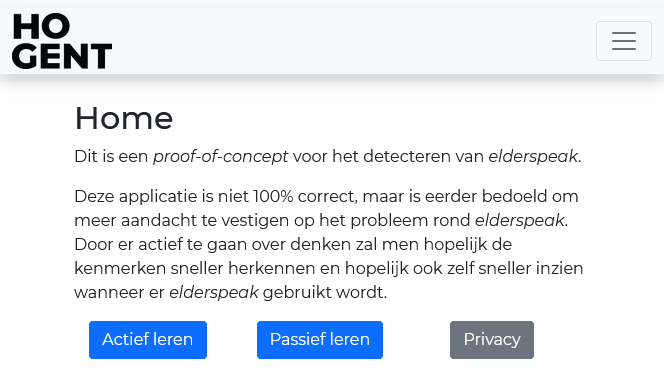
\includegraphics[width=1\textwidth]{./img/home_website}
    \caption{\label{fig:home_page} Home pagina website}
\end{figure}


\begin{figure}
    \centering
    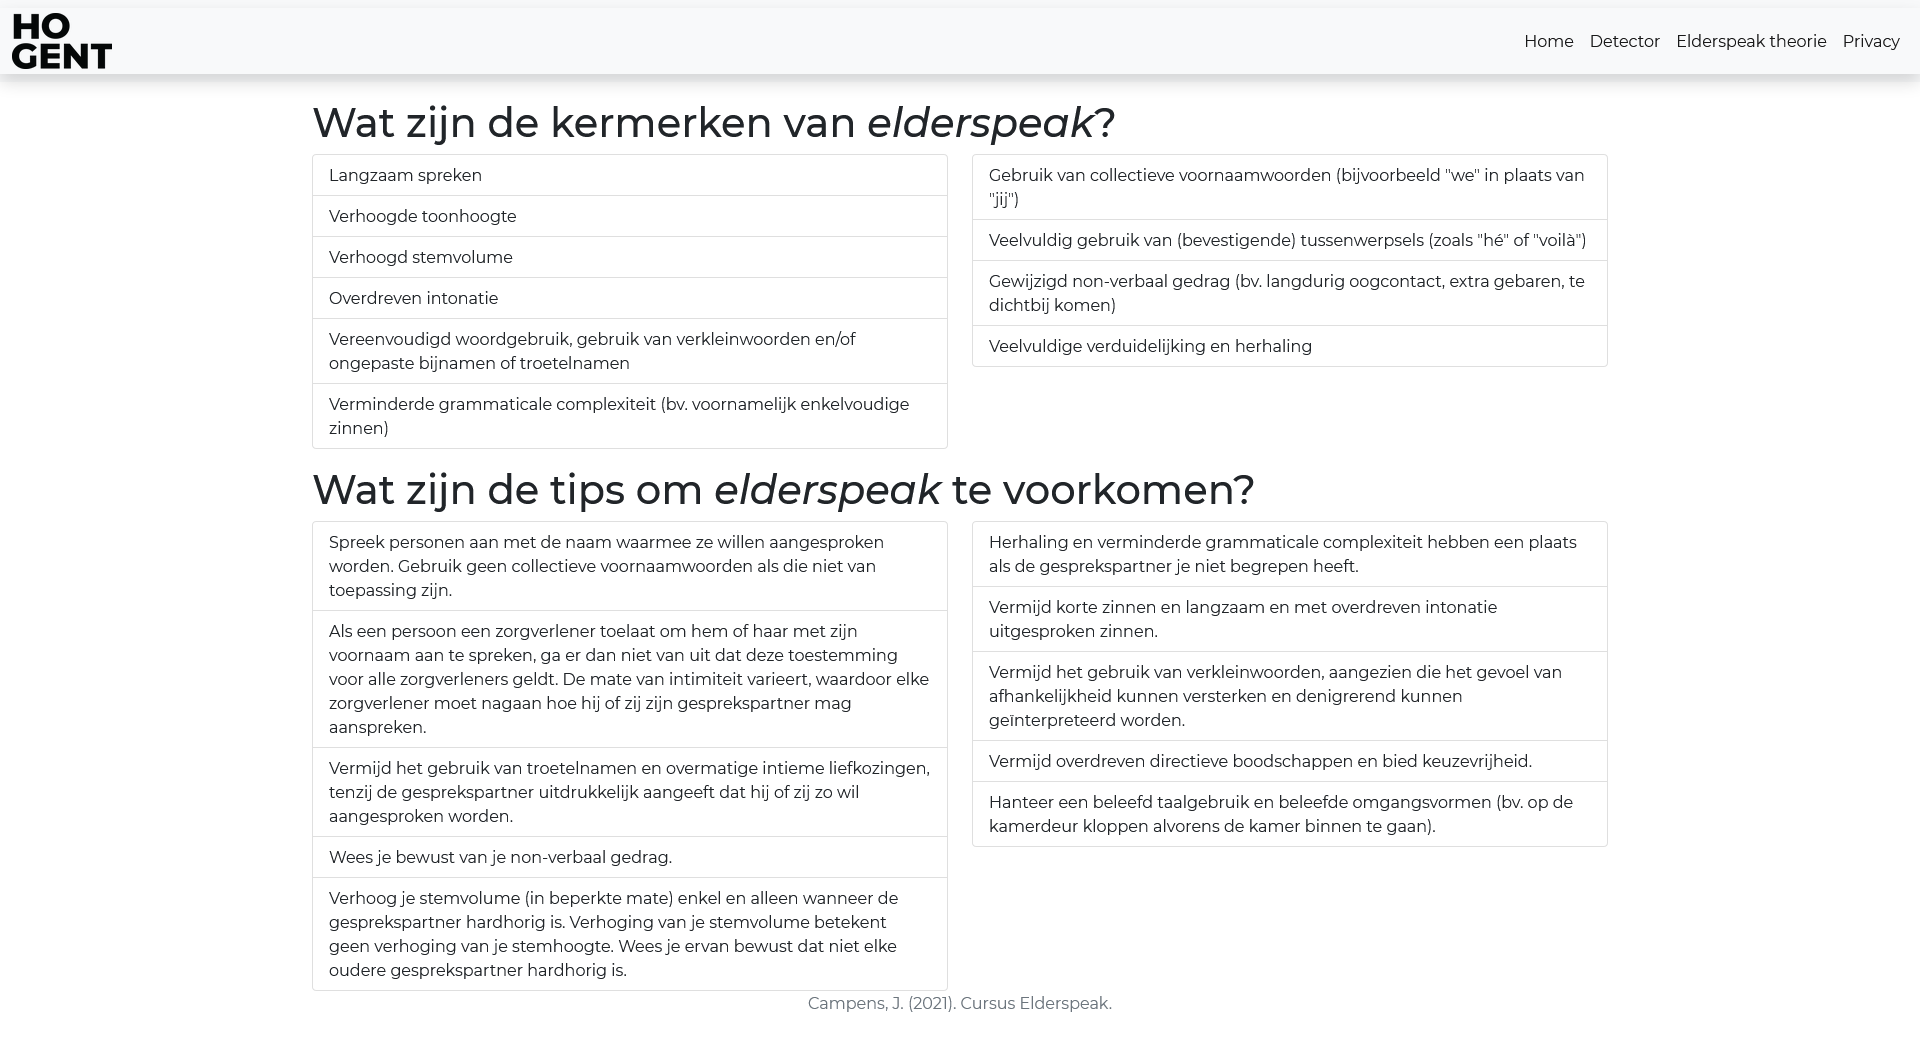
\includegraphics[width=1\textwidth]{./img/eigenschappen_elderspeak_website}
    \caption{\label{fig:eigenschappen_page} Eigenschappen \textit{elderspeak} op de website}
\end{figure}

\begin{figure}
    \centering
    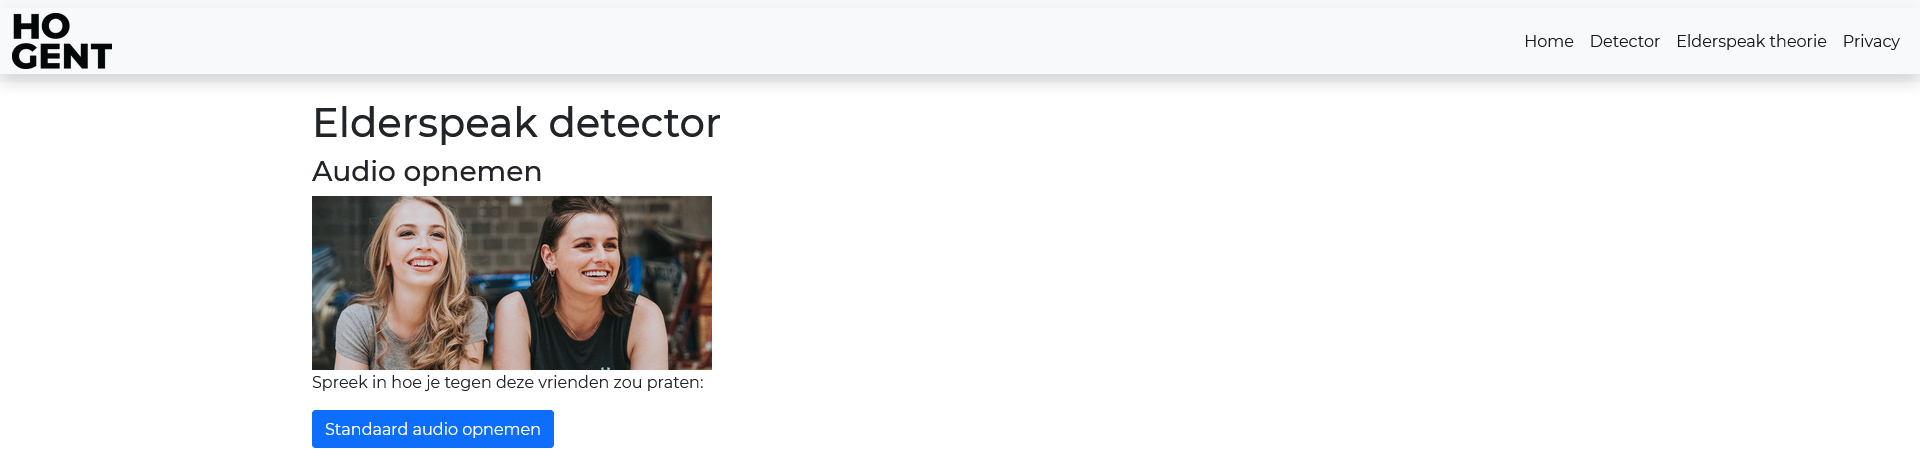
\includegraphics[width=1\textwidth]{./img/detector_begin_elderspeak}
    \caption{\label{fig:detector_begin_page} Detector bij het begin}
\end{figure}

\begin{figure}
    \centering
    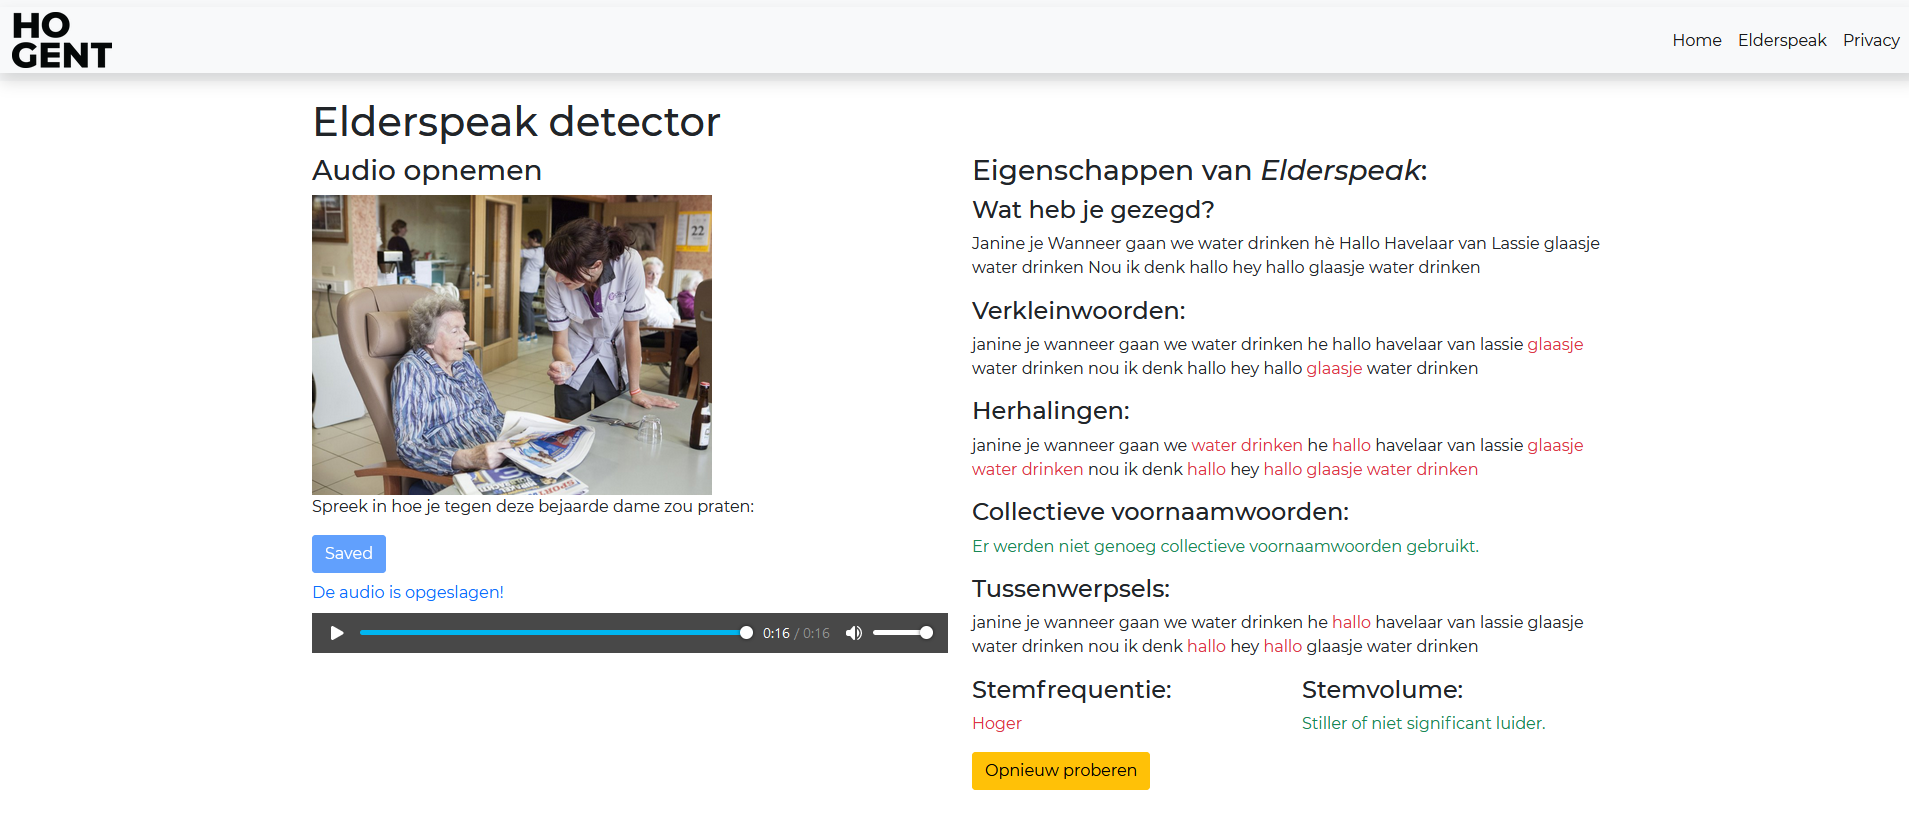
\includegraphics[width=1\textwidth]{./img/dector_na_detecteren}
    \caption{\label{fig:detector_end_page} Detector na het analyseren}
\end{figure}


\subsection{\textit{Speech recognition}}
De basis van een groot deel van de applicatie is het herkennen van de spraak die wordt opgenomen op de website. Uiteraard moet dit niet van nul gemaakt worden, maar kan er gebruik gemaakt worden van een bestaande Python-bibliotheek. \textcite{Standaert2021} bestudeerde in zijn bachelorproef afgelopen jaar dat de beste optie is om de Google Speech Recognition-API te gebruiken omdat deze het beste presteert. Hij vatte dit samen in zijn conclusie: ``Uit verschillende onderzoeken of studies waar men verschillende ASR-systemen met elkaar vergeleken kwam de Google Speech-API er altijd als beste uit. En dit in alle aspecten.''. Daarnaast gebruikt de Google Speech-API ook \textit{natural language processing} of NLP om beter te kunnen weten wat er precies gezegd is geweest~\autocite{GoogleCloud2022}. Hoe dit precies in elkaar zit is te lezen in het literatuuronderzoek, namelijk in Hoofdstuk~\ref{ch:stand-van-zaken}.

Bij de spraakherkenning kwam er wel een groot probleem de kop op steken. De Google \textit{Speech Recognition}-API kon alleen overweg met \textit{wav}- en \textit{flac}-bestanden én kan maar een bepaalde periode, ongeveer 2 tot 3 minuten, gratis herkennen. Het probleem is dus dat de audio gecapteerd is in een \textit{mp3}-formaat. Hiervoor was het noodzakelijk om eerst een conversie te maken van \textit{mp3} naar \textit{flac} en om het audiobestand op te delen in deelbestandjes of \textit{chuncks}, zodat er geen betalende versie voor nodig was. De gebruikte technologie hierbij was ``ffmpeg''. Hoe de conversie precies gebeurt is te vinden tot in detail in bijlage~\ref{bijlage:speech_recognition}.

Het gebruiken van die API is relatief gemakkelijk. Een extra optie is dan ook ter beschikking om achtergrondlawaai een beetje weg te filteren. Door de optie \newline`ajust\_for\_ambient\_noice(source)' aan te zetten, zal de bibliotheek zich wat aanpassen aan de geluidsbron zodat het beter de klanken kan horen alvorens die worden doorgestuurd naar de spraakherkenning-API. Deze methode gebruikt de techniek die beschreven is in het literatuuronderzoek over achtergrondlawaai.

Eens dit ingesteld is, worden de audiobestanden mee gegeven en krijgt het systeem de tekst terug waarvan het AI-model van Google de tekst herkend heeft. Uiteraard werkt dit niet feilloos, maar het is wel redelijk goed voor een gratis versie. Met deze grotere methode is de basis gelegd voor andere methoden die steunen op de tekst die herkend werd.

\subsection{Verkleinwoorden}
Voor de methode om verkleinwoorden te herkennen is er gefundeerd op de methode van \textcite{Standaert2021}. Daarbij wordt er gekeken of woorden langer zijn dan 3 letters en ze niet voorkomen in de lijst die geen verkleinwoorden zijn. Enkele voorbeelden die wel eindigen op ``-je'', ``-ke'', ``-kes'' of ``-jes'', maar voorbeelden die geen verkleinwoorden zijn, zijn: poffertje, meisje, koopje, etentje, dutje, toetje, mannelijke, vrouwelijke etc. De code voor deze methode kan gevonden worden in bijlage~\ref{bijlage:verkleinwoorden}.

\subsection{Herhalingen}
Om herhalingen te herkennen werd er evenals gebruikt gemaakt van de methode die \textcite{Standaert2021} geschreven had. Daarbij wordt er bijgehouden wat de vorige 25 woorden waren en bij herhalingen worden de woorden die herhaald worden bewaard in een lijst. Die zullen we later gebruiken om een mooie weergave te maken.
De code om herhalingen te detecteren is te vinden in bijlage~\ref{bijlage:herhalingen}.

\subsection{Collectieve voornaamwoorden}
Een voorbeeld van een collectief voornaamwoord is het gebruiken van: ``we'' / ``wij''. Om het voorbeeld te verduidelijken zijn de volgende zinnen gegeven: ``Gaan we onze patatjes opeten?'', ``Kunnen we alleen naar de wc?'', ``Awel, wat zijn we aan het doen?''.

Er wordt bijgehouden hoeveel keer er collectieve voornaamwoorden gebruikt worden in de tekst. Als een woord meer dan een keer voorkomt, dan beschouwt de applicatie dit dat het voorkomt. Dit is zo ingesteld omdat het niet mag worden weergegeven wanneer er iemand een keer het woord ``we'' gebruikt.
Wanneer er geen of minder dan twee collectieve voornaamwoorden gebruikt worden, zal de applicatie zeggen dat er geen of niet genoeg gebruikt werden.

Natuurlijk duiden twee of meer collectieve voornaamwoorden niet direct op \textit{elderspeak}, maar het geeft wel al een richting. De persoon in kwestie moet natuurlijk de theorie over \textit{elderspeak} weten en moet daarna ook kritisch zijn over het resultaat en dit kan via een zelfreflectie.

\subsection{Tussenwerpsels}
Het veelvuldig gebruik van tussenwerpsels is een eigenschap van \textit{elderspeak} en ook dit wordt herkend. Enkele voorbeelden van tussenwerpsels die herkend worden zijn: ``o'', ``oeps'', ``helaas'', ``hallo'', ``hey'', ``voila'' etc. De Google \textit{Speech Recognition}-API geeft soms verschillende varianten op het woord ``hey''. Zo worden de volgende vormen soms gegeven: ``hé'', ``hè'', ``he'', ``hey''. Om te voorkomen dat dat foute resultaten oplevert, worden al deze varianten herleid naar ``hey''.

De werkwijze om dit te detecteren is ongeveer dezelfde als bij de methode van de collectieve voornaamwoorden die te vinden is in bijlage~\ref{bijlage:tussenwerpsels}.

\subsection{Toonhoogte}
De toonhoogte is een bijzonder belangrijke eigenschap van \textit{elderspeak}. Deze eigenschap is ook volledig onafhankelijk van de gesproken tekst die herkend werd. Wanneer een persoon merkbaar hoger zal praten, zal de andere persoon direct voelen dat hij/zij behandeld wordt als een kind. Het is dan ook belangrijk dat deze functie goed werkt zodat de gebruikers direct weten wanneer ze (on)bewust hoger praten.

Deze methode werd al opgesteld door \textcite{Standaert2021} in zijn eindwerk van het vorige jaar. Wat hij berekende was de gemiddelde toonhoogte, uitgedrukt in Hz, van het gegeven audiobestand. Wat er aan deze applicatie toegevoegd is, is het berekenen of de toonhoogte hoger ligt bij de casus met de oudere vrouw dan de casus bij de twee jonger vrouwen.
Hoe dit gerealiseerd werd in de code is te vinden in bijlage~\ref{bijlage:toonhoogte}.

\subsection{Stemvolume}
De laatste eigenschap die geanalyseerd wordt in de applicatie is om te controleren of er luider gesproken wordt in het 2\textsuperscript{e} fragment dan in het 1\textsuperscript{ste}. Toch moet er hier een duidelijke kanttekening bij gemaakt worden. Wanneer een persoon bij de 2\textsuperscript{e} opname significant verder van de microfoon staat, zal de applicatie dit detecteren dat het niet luider zal zijn. Daarnaast moet er ook geweten zijn dat de meeste oudere mensen slechthorend zijn, waardoor men wel luider moet praten. Ondanks deze twee zaken vond ik het toch belangrijk om deze eigenschap te implementeren zodat men er wel eens bij stil staat dat niet iedereen slechthorend is of een hoorapparaat draagt.

Om een getal te verkrijgen dat het volume voorstelt, is er gebruik gemaakt van de pyln-bibliotheek die een BS.170 geluidsmeter aanmaakt in de code. Deze analyseert dan de audio en geeft een getal weer. Hoe dit precies geïmplementeerd werd is te vinden in bijlage~\ref{bijlage:stemvolume}.

\section{\textit{Front-end}}
\subsection{Geluid opnemen}
Het geluid opnemen gebeurt volledig aan de kant van de \textit{client} of de gebruiker. Wanneer er op de knop geduwd wordt om de audio-opname te starten, zullen er \textit{audiochunks } worden toegevoegd aan een lijst. Die worden na de opname allemaal samengevoegd tot een \textit{blob}, of een \textit{binary-large object}, die dan een \textit{mp3}-file aanmaakt.
Per casus wordt er ook een andere afbeelding en tekst getond boven de opneemknop.

\subsection{API-afhandeling}
Vanuit de front-end worden er \textit{API-requests} gestuurd met het audiobestand als bijlage naar de \textit{back-end}. De server analyseert dan de verschillende methodes. Wanneer alles onderzocht is, wordt alle data verzameld en via een JSON-formaat terug gestuurd naar de \textit{client}. Daar worden de resultaten ingevuld in de voorziene html-stukken.

\section{Testen}
Om een objectief beeld te kunnen verkrijgen hoe goed de applicatie werkt, zijn er automatische testen opgezet. De data die verzameld is via een online formulier, is te vinden op:  \url{https://www.jotform.com/form/213524968382060}. Deze werd in het begin van het twee semester verzameld. Eens de data opgeslagen was werd alle data beluisterd en handmatig gelabeld.

Nadien werd er een Python-script gemaakt die het testen van al die 54 bestanden automatiseerde. De audiobestanden die geklasseerd werden, waarbij er geen \textit{elderspeak} aanwezig bij was, werden gebruikt zoals in de echte webapplicatie om eerst een normaal stukje audio te hebben. Zo kan er toch vergelijken worden met een normale spraak en de spraak die erna komt. Nadien werden de geluidsopnames,  waarbij er wel \textit{elderspeak} bij aanwezig was, gebruikt voor het te testen van de applicatie zelf. De resultaten werden dan vergeleken met de gelabelde data.

Met deze resultaten konden er over de eigenschappen verkleinwoorden, hogere toonhoogte en hoger volume, een \texit{confusion matrix} gemaakt worden. Hierbij wordt er bepaald hoeveel correct negatieve, correct positieve, valse positieve en vals negatieve er aanwezig waren in het testset. Dit wordt dan in een matrix gegoten die visueel te vinden is in figuur~\ref{fig:confusion_matrix}. De resultaten daarvan zijn te vinden in het resultatenhoofdstuk, namelijk Hoofdstuk~\ref{ch:resultaten}.

\begin{figure}
    \centering
    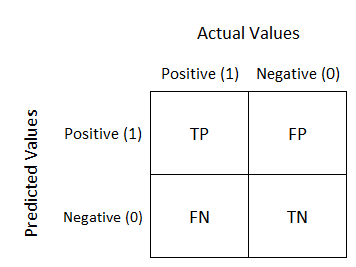
\includegraphics[width=0.6\textwidth]{./img/confusion_matrix}
    \caption{\label{fig:confusion_matrix} Confusion Matrix~\autocite{Jain2020}}
\end{figure}


% Voeg hier je eigen hoofdstukken toe die de ``corpus'' van je bachelorproef
% vormen. De structuur en titels hangen af van je eigen onderzoek. Je kan bv.
% elke fase in je onderzoek in een apart hoofdstuk bespreken.

%\input{...}
%\input{...}
%...

%%=============================================================================
%% Conclusie
%%=============================================================================

\chapter{Conclusie}
\label{ch:conclusie}

% Trek een duidelijke conclusie, in de vorm van een antwoord op de
% onderzoeksvra(a)g(en). Wat was jouw bijdrage aan het onderzoeksdomein en
% hoe biedt dit meerwaarde aan het vakgebied/doelgroep?
% Reflecteer kritisch over het resultaat. In Engelse teksten wordt deze sectie
% ``Discussion'' genoemd. Had je deze uitkomst verwacht? Zijn er zaken die nog
% niet duidelijk zijn?
% Heeft het onderzoek geleid tot nieuwe vragen die uitnodigen tot verder
%onderzoek?

Uit deze bachelorproef kan besloten worden dat \textit{elderspeak} of \textit{nursery tone} onrechtstreeks kan gedetecteerd worden met artificiële intelligentie. Het verkozen type AI is verwerkt in de Google \textit{Speech Recognition}-API. Op basis van die spraakherkenning wordt er gedetecteerd of verkleinwoorden, herhalingen, collectieve voornaamwoorden en/of tussenwerpsels aanwezig zijn. Daarnaast worden ook de toonhoogte en het stemvolume berekend via Python-bibliotheken die geen gebruik maken van kunstmatige intelligentie.

Het type model dat de Google \textit{Speech Recognition}-API gebruikt, is natuurlijk niet zomaar online terug te vinden. Het is wel algemeen bekend dat Google aan \textit{natural language processing} doet.
Het achtergrondlawaai kan gemakkelijk worden weggefilterd via de volgende methode in de Google \textit{Speech Recognition}-API: `ajust\_for\_ambient\_noice(source)'.

Spraakherkenning in Python is mogelijk via een gratis softwarebibliotheek, mits enkele aanpassingen. Zo is het noodzakelijk om \textit{wav}- en \textit{flac}-bestanden van de audio te hebben. Met andere formaten kan de bibliotheek niet overweg. Gratis gebruik van de software is ook gelimiteerd. Wanneer het geluidsbestand langer is dan 2 à 3 minuten, geeft de API een foutboodschap. Wanneer het geluid opgedeeld wordt in deelbestandjes of \textit{chunks} lukt het wel.

Het opzetten van een ``Flask applicatie'' is bijzonder simpel. Het is een goede manier om snel een webserver op te zetten in Python. Het model ermee verbinden of, in ons geval, de methoden aanroepen, is ook eenvoudig. Er kan gemakkelijk een ander bestand dat alle berekeningen heeft, geïmporteerd worden.

Om te kunnen staven dat \textit{elderspeak} goed gedetecteerd kan worden, is er nood aan meer testgevallen. Zo is het momenteel nog niet volledig duidelijk of de methoden die de toonhoogte en het stemvolume bepalen, goed genoeg werken. Wat de mogelijke vervolgopdrachten of -studies zijn, is te vinden in Hoofdstuk~\ref{ch:vervolg}.

\section{Discussie}
In deze discussie wordt besproken of het nuttig is voor verpleegkundigen om deze applicatie in gebruik te nemen.

Concluderend kunnen we stellen dat deze applicatie zeker en vast gebruikt kan worden voor studenten in de zorgsector. Op die manier kunnen ze \textit{elderspeak} ontdekken en het fenomeen beter leren herkennen. Dat kan zowel actief, via de detector, als passief, door de lijst van eigenschappen en tips te lezen.

De accuraatheid is niet ideaal, maar dat hoeft ook niet. Wanneer iemand de detector gebruikt, is het belangrijk dat hij of zij ook aan zelfreflectie doet. Op die manier blijven het begrip en de eigenschappen langer aanwezig in het geheugen.

Met alle argumenten die aangehaald zijn in deze tekst, kan er toch wel besloten worden dat deze applicatie nuttig zal zijn in de toekomst. Hopelijk wordt de website wel degelijk ingezet tijdens de lessen \textit{elderspeak} in de richting verpleegkunde.

%%=============================================================================
%% Bijlagen
%%=============================================================================

\appendix
\renewcommand{\chaptername}{Appendix}

%%---------- Onderzoeksvoorstel -----------------------------------------------

\chapter{Onderzoeksvoorstel}

Het onderwerp van deze bachelorproef is gebaseerd op een onderzoeksvoorstel dat vooraf werd beoordeeld door de promotor. Dat voorstel is opgenomen in deze bijlage.

% Verwijzing naar het bestand met de inhoud van het onderzoeksvoorstel
% Voor literatuurverwijzingen zijn er twee belangrijke commando's:
% \autocite{KEY} => (Auteur, jaartal) Gebruik dit als de naam van de auteur
%   geen onderdeel is van de zin.
% \textcite{KEY} => Auteur (jaartal)  Gebruik dit als de auteursnaam wel een
%   functie heeft in de zin (bv. ``Uit onderzoek door Doll & Hill (1954) bleek
%   ...'')

%---------- Inleiding ---------------------------------------------------------

\section{Introductie}\label{sec:introductie} % The \section*{} command stops section numbering

De veroudering van de bevolking in de Vlaamse steden en gemeenten zet zich in de komende  decennia verder.~\autocite{StatistiekVlaanderen2018}
Volgens hun voorspellingen zou tegen 2033 25\% van de bevolking een 65-plusser zijn.

Het woord `waardigheid' is actueler dan ooit.
Na de schrijnende omstandigheden van de Tweede Wereldoorlog stond dat woord centraal bij het opstellen van het verdrag van de Verenigde Naties (1945), de Universele Verklaring van de Rechten van de mens (1948) en de grondrechten van de Europese Unie (2000).
Die basiswaarde vinden we ook terug bij het Europese en Belgische zorgbeleid. Ouderen mogen niet gediscrimineerd worden op vlak van leeftijd. Tevens mogen ze ook niet op een kinderlijke, betuttelende of onvriendelijke wijze aangesproken worden en moeten ze met respect bejegend worden~\autocite{Campens}.

Hoe meer ouderen er in de samenleving zijn, hoe meer zorg zij nodig hebben en hoe meer zorgverleners instaan voor deze leeftijdscategorie.
Die zorgverleners, maar evengoed familie, weten niet altijd even goed hoe ze moeten omgaan met senioren.
Wanneer een jonger persoon op een andere manier spreekt tegen een senior dan tegen een leeftijdsgenoot, spreken we over \textit{elderspeak}. \textcite{Williams2011} omschrijft \textit{elderspeak} als volgt: ``Elderspeak is a common intergenerational speech style used by younger persons in communication with older adults in a variety of community and health care settings. Based on negative stereotypes of older adults as less competent communicators, younger speakers (in this case nursing home staff) modify their communication with nursing home residents by simplifying the vocabulary and grammar and by adding clarifications such as repetitions and altered prosody.'' Om \textit{elderspeak} te bestrijden, gaven \textcite{Wick2007} een paar tips mee in hun onderzoek.
Enkele van die tips gingen als volgt: spreek mensen aan zoals ze wensen aangesproken te worden, vraag om ze aan te spreken met de voornaam, vermijd troetelnamen, wees bewust van non-verbaal gedrag, verhoog uw stemvolume enkel wanneer uw gesprekspartner hardhorig is, herhaal alleen uw zin als uw gesprekspartner het niet begrepen heeft, vermijd korte, langzame en makkelijke zinnen, vermijd verkleinwoorden en hanteer beleefd taalgebruik.

Naast \textit{elderspeak} heb je ook nog \textit{nursery tone}. Dit verwijst naar de situatie waarbij iemand de toonhoogte aan het einde van de zin standaard verhoogt zoals bij communicatie met jonge kinderen.

Dit onderwerp was vorig jaar al een onderzoeksonderwerp voor Glenn~\textcite{Beeckman2021} en Victor~\textcite{Standaert2021}.
Zij hebben al een basis gelegd in de goede richting om dit project tot een goed einde te brengen.
Sommige stukken programmacode van hen zullen gebruikt worden om zo een beter model op te stellen.
Zij haalden zelf ook verbeterpunten aan en moeilijkheden die, hopelijk, op te lossen zijn. Wat het verschil zal zijn tussen hun eindwerken en dit eindwerk wordt toegelicht in \ref{sec:state-of-the-art}.

De nog steeds relevante onderzoeksvraag van dit onderwerp is: ``Kan \textit{elderspeak} gedetecteerd worden door Artificiële Intelligentie en kan dit toegepast worden in de praktijk?''. Een bijkomende onderzoeksvraag is: ``Kan \textit{nursery tone} gedetecteerd worden door Artificiële Intelligentie?''.

Met dit eindwerk zal ik alle mogelijkheden en capaciteiten van mezelf inzetten om een applicatie én AI-model te maken zodat dit kan getest en gebruikt worden in de opleiding verpleegkunde.
Ik hoop ook dat ik ouderen op deze manier een betere levenskwaliteit kan bieden door de communicatie met zorgverleners, en misschien zelfs hun familie, te optimaliseren.


%---------- Stand van zaken ---------------------------------------------------

\section{State-of-the-art}
\label{sec:state-of-the-art}

\subsection{Literatuuronderzoek}\label{subsec:literatuuronderzoek}

Omdat voorgaande studenten al uitgezocht hebben wat \textit{elderspeak} precies is, zal dit niet herhaald worden in dit onderzoek.
Wel zal er op basis van de beschikbare literatuur onderzocht worden welk soort machinaal leren of \textit{deep learning} het meest geschikt is voor deze specifieke taken. Zowel \textit{machine learning} als \textit{deep learning} hebben elk verschillende onderlinge modellen. Er moet dan bekeken worden welke hypothese het beste past om bovenstaande parameters te integreren in het model of verschillende modellen.

Een extra obstakel kan verschijnen wanneer er te veel achtergrond lawaai aanwezig is. Mogelijks moet er dan eerst een filter worden toegepast op de audiobestanden om dit weg te filteren zodat deze wel gebruikt kunnen worden voor het herkennen van eigenschappen op \textit{elderspeak}.

\subsection{Stand van zaken}\label{subsec:stand-van-zaken}

Zoals reeds vermeld in de inleiding werd dit bachelorproef-onderwerp vorig jaar al gekozen door twee studenten.
Zij hebben zich gefocust op de \textit{speech-to-text}, verkleinwoorden detecteren, een frequentiemeter, herhalende zinnen herkennen, emotie-herkenner en een basisapplicatie in `Tkinter', een standaard \textit{Graphical User Interface} (GUI) in Python.

\textcite{Beeckman2021} vermeldde dat er nog nood was aan een methode om herhaling en verkleinwoorden te detecteren. ~\textcite{Standaert2021} haalde aan dat er nog onderzoek nodig was voor de spraakherkenning en de frequentiemeter om de applicatie preciezer te maken.

\subsection{Wat is mijn aandeel?}\label{subsec:watismijnadeel}

Beide studenten hebben niet echt Kunstmatige Intelligentie gebruikt om het resultaat te bekomen. \textcite{Standaert2021} heeft wel methoden beschreven om een paar kenmerken te herkennen, maar dit gebeurt op basis van vaste parameters.
Mocht AI gebruikt kunnen worden om de nauwkeurigheid op te schalen, dan zou dat alvast een winst zijn.
Het gebruik van Machinaal leren of \textit{Deep Learning}, meer specifiek een \textit{Convolutional Neural Network} (CNN) kan een positief effect hebben op het detecteren van alle parameters rond \textit{elderspeak}. Mijn aandeel zal dus zijn om te onderzoeken welke modellen het beste gebruikt worden om die parameters te detecteren.

Een belangrijke stap zal zijn om de twee eerder vernoemde eindwerken samen te voegen en te verbeteren. \textcite{Beeckman2021} gebruikte ``Tkinter'' om de \textit{front-end} te maken, maar haalde een paar redenen aan waarom dat toch niet te verkiezen is, zoals bijvoorbeeld het amateuristische uiterlijk en de beperkte mogelijkheden.
Mijn voorkeur gaat eerder uit naar het gebruik van ``Flask'', een \textit{micro-webframework} in Python, dat kan gebruikt worden om een webpagina te maken en te linken naar de \textit{back-end}.
Het voordeel hiervan is dat men sneller én mooier een website kan ontwerpen.


%---------- Methodologie ------------------------------------------------------
\section{Methodologie}
\label{sec:methodologie}

Om te verzekeren dat er genoeg data beschikbaar is, is het aan te raden dat er audiosamples verzameld worden voor het 2\textsuperscript{e} semester.

Op basis van de resultaten van het literatuuronderzoek en beide eindwerken van vorig jaar, kunnen er methodes opgesteld worden die de belangrijkste kenmerken van \textit{nursery tone} en \textit{elderspeak} herkennen.
Daarbij is het gebruik van Artificiële Intelligentie een handige manier om het verschil te kennen tussen iemand die \textit{elderspeak} gebruikt en iemand die dat niet doet. Met welk model en op welke wijze dit het beste gerealiseerd wordt, zal onderzocht worden in dit eindwerk.

Daarnaast moet alles omgezet worden naar een duidelijke webapplicatie via ``Flask'' zodat het in latere fases niet geïnstalleerd moet worden op een computer. Zo kan iedereen de applicatie gebruiken zonder vooraf iets te downloaden, wat het gebruiksgemak thuis en op verplaatsing, bijvoorbeeld in een rusthuis, optimaliseert.

Tot slotte zullen het beantwoorden van de volgende deelvragen hierbij moeten helpen:
\begin{itemize}
	\item Welk type Artificiële Intelligentie past het beste bij deze opstelling?
	\item Welk type model van \textit{machine learning} of \textit{deep learning} werkt het beste per eigenschap?
	\item Kan je achtergrond lawaai wegfilteren en hoe precies?
	\item Zal spraakherkenning lukken met de gratis beschikbare softwarebibliotheken?
	\item Hoe zet je een ``Flask'' server op waar je \textit{webrequests} naar stuurt? En hoe verbind je daar een model mee?
\end{itemize}


%---------- Verwachte resultaten ----------------------------------------------
\section{Verwachte resultaten}
\label{sec:verwachte_resultaten}

Het verwachte resultaat is een webapplicatie met ``Flask'' als \textit{back-end}, waarbij men de optie heeft om het model te trainen, en waarbij het model aangeeft of er \textit{elderspeak} of \textit{nursery tone} aanwezig is. Bovendien geeft de applicatie weer op basis van welke parameters het model `denkt' dat het om die twee taalregisters gaat.

%---------- Verwachte conclusies ----------------------------------------------
\section{Verwachte conclusies}
\label{sec:verwachte_conclusies}

De gehoopte resultaten houden in dat er een meetbaar verschil is tussen personen die \textit{nursery tone} gebruiken t.o.v.\ mensen die normaal praten.
Het model zal nooit 100\% accuraat zijn: zo spreekt men in de praktijk vaker dialect tegen ouderen terwijl de algoritmes getraind zijn op Algemeen Nederlands (AN), en ook het verschil tussen de Nederlandse uitspraak en de Vlaamse uitspraak kunnen een obstakel vormen.
Ook het filteren van achtergrondlawaai wordt een bijkomende uitdaging.



%%---------- Andere bijlagen --------------------------------------------------
% TODO: Voeg hier eventuele andere bijlagen toe
%\input{...}

%%---------- Referentielijst --------------------------------------------------

\printbibliography[heading=bibintoc]
 
\end{document}
